%------------------------------------------------------------------------------
\section{Results}

During the course of the analysis, results were inspected using \ac{PT} and using \ac{QE} for bias correction.
The plots were similar in distribution, and each gave a similar magnitude for the information.
However, \ac{PT} gave visibly lower variance than \ac{QE}, so only plots using \ac{PT} are presented in this results section.

Using the $I_{\text{sh}}$ approach where the bias is corrected by shuffling bins across trials \citep{Montemurro2007} was also attempted for the spike timing code, but this increased the variance far too much to be of any practical use.
The unexpectedly significant increase in variance is probably due to the nature of the correlations between the bins which are being shuffled.

We also compared some of the results both with the monitor artifact left in the data and with the dataset redacted to have it removed.
There was no appreciable difference for any of the plots, though the amount of information went down when the data was redacted due to the loss of some of the spikes.


%------------------------------------------------------------------------------
% \FloatBarrier
% \subsection{General Information plots}

Starting with \ac{V1}, the first thing which is noticed in Figs.~\ref{fig:b1-trialwise} and \ref{fig:j1-trialwise} \ref{fig:b1-1x20tp4} and \ref{fig:b1-5x4tp4} is the large peak in information over the \SI{20}{ms} window starting at around \SI{40}{ms} after stimulus onset.
This is due to the onset transient response, where there is a larger amount of neural activity, and this is also less variable than usual \citep{Muller2001}.
A second, smaller peak from the ``rebound'' of the transient also occurs around \SI{100}{ms} after stimulus onset.
Looking at the scale bars, we can see there is about 10 times as much information on average from the neurons in \ac{M2} than \ac{M1}.
This is probably due to differences in data quality between the two animals.

Comparing the information found using the spike timing code \ref{fig:b1-5x4tp4} with the spike count code \ref{fig:b1-1x20tp4}, it seems that there is significantly more information when the binned spike times are considered: there is three times as much information for the spike timing code for \ac{M1} and twice as much for \ac{M2}.
However, if we look at information in the spontaneous activity, this reveals we cannot trust this result, as the bias for the information from the spontaneous activity is much higher for the spike timing code than spike count.

For \ac{M1}, aside from the transient, the information measured with the spike timing code from the spontaneous activity is about the same as the information from the test presentation, suggesting something has gone very wrong!

For the spike timing codes, there is a clear decrease in information with learning in \ac{M1}, and a clear increase in information for \ac{M2}.
This is, however, present in both the test presentation activity and the spontaneous activity, suggesting it is not a genuine effect.
This is believed to be due to a decrease in signal quality in the implants in \ac{M1}, and possibly an increase in \ac{M2}.
The increase is also seen in the spike count code for \ac{M2}, but not to any real extent and it is doubtful that the result is significant.

The bias in the information for the spontaneous activity changes with time for the spike timing code, but does not for the spike count code.
Since any changes in the dataset are the same for both of these, this suggests there are too few trials for the spike timing code to give a reliable reading of the information.
This would make sense because with an average of $N_S = 100$ trials per stimulus and a spike timing code with $\overline{R} = 32$, there are
on average $\nicefrac{N_S}{\overline{R}} = 3.125$ trials per response per stimulus,
whilst for a spike count code with $\overline{R} = 8$ there are on average $\nicefrac{N_S}{\overline{R}} = 12.5$ trials per response per stimulus.
Similarly if there we assume a minimum of $N_S = 64$ trials per stimulus, there are
at least $\nicefrac{N_S}{\overline{R}} > 2$ trials per response per stimulus for the spike timing code, and
at least $\nicefrac{N_S}{\overline{R}} > 8$ trials per response per stimulus for the spike count code.

The information in the spontaneous activity was subsequently computed with an average of $N_S = 200$ and with $N_S = 400$ trials per stimulus.
This means there is now $\nicefrac{N_S}{\overline{R}} > 8$ for the spike timing code, however precisely the same relationship was observed.
From this, we can conclude the problem is due to the inconsistencies between sessions.
If the firing rate changes between two sessions, the probability distribution of the responses generated will change for each condition.
This will not matter so much for the spike count code because there are only 8 possible responses, and even if there are only 250 trials in the session there should be at least 16 trials per condition, meeting the minimal requirements for the \ac{PT} method to function.

The small bump in the information in the spontaneous activity around \SI{50}{ms} in Figs.~\ref{fig:b1-5x4tp4} and \ref{fig:j1-5x4tp4} will be due to an increase in activity from a transient response.
This data is normalised so \SI{0}{ms} is when the animal begins fixating on the fixation target, and there will be a transient response after the animal saccades to the target.
Although the increase in activity does not relate to the conditions used on the subsequent test presentation, the extra spikes will increase the variability of the response, and thus $H(\SET{R})$, which will not be cancelled out by an increase in $H(\SET{R}|\SET{S})$ for the same reasons the bias appears in the first place.

In short, the data for \ac{M1} \ac{V1} does not seem to be of good enough quality whilst \ac{M2} \ac{V1} does, and the information in the spike timing code cannot be trusted for either monkey.

%  figs/info/I_trialwise_blanco_v1_chmean23_s343-354,355.1,355.2,356-359_tp4_1bins_of_20ms_dr_pt_oc0_test_tc5-5-20,22-3-28,32,35-5-50,60,90_nt1400_ts350_rmvet1_rmvms0_pcolorhot_20120815T234452.png
% figs/info/I_trialwise_blanco_v1_chmean23_s343-354,355.1,355.2,356-359_tp1_1bins_of_20ms_dr_pt_oc0_test_tc5-5-20,22-3-28,32,35-5-50,60,90_nt1400_ts350_rmvet1_rmvms0_pcolorhot_20120815T234326.png
% figs/info/I_trialwise_blanco_v1_chmean23_s343-354,355.1,355.2,356-359_tp4_1bins_of_20ms_dr_pt_oc0_test_tc5-5-20,22-3-28,32,35-5-50,60,90_nt1400_ts350_rmvet1_rmvms1_pcolorhot_20120815T234741.png
% figs/info/I_trialwise_blanco_v1_chmean23_s343-354,355.1,355.2,356-359_tp1_1bins_of_20ms_dr_pt_oc0_test_tc5-5-20,22-3-28,32,35-5-50,60,90_nt1400_ts350_rmvet1_rmvms1_pcolorbp_20120816T175451.png
% figs/info/I_trialwise_blanco_v1_chmean23_s343-354,355.1,355.2,356-359_tp4_5bins_of_4ms_dr_pt_oc0_test_tc5-5-20,22-3-28,32,35-5-50,60,90_nt1400_ts350_rmvet1_rmvms1_pcolorhot_20120815T234513.png
% figs/info/I_trialwise_blanco_v1_chmean23_s343-354,355.1,355.2,356-359_tp1_5bins_of_4ms_dr_pt_oc0_test_tc5-5-20,22-3-28,32,35-5-50,60,90_nt1400_ts350_rmvet1_rmvms1_pcolorbp_20120816T175423.png

% % \cleartoevenpage

% % \begin{figure}[htbp]
% % %     \begin{subfigure}[b]{0.5\linewidth}
% % %         \centering
% % %         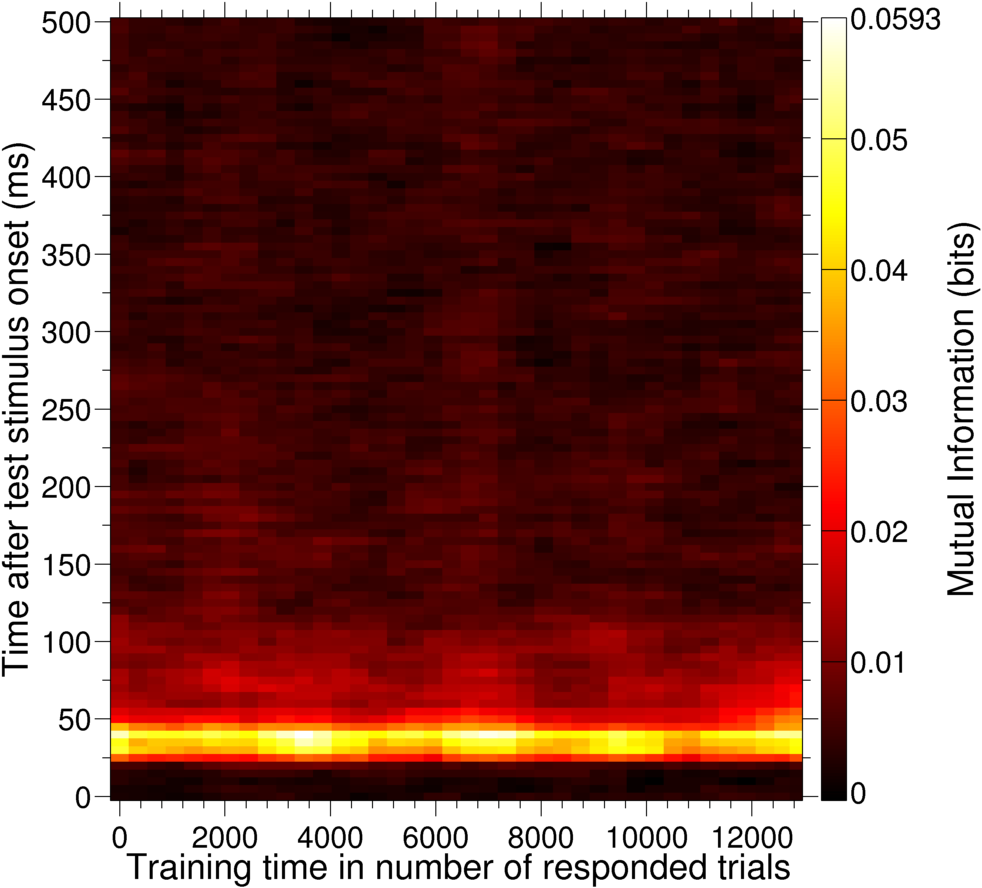
\includegraphics[scale=.25]{%
% % % figs/info/I_trialwise_blanco_v1_chmean23_s343-354,355.1,355.2,356-359_tp4_1bins_of_20ms_dr_pt_oc0_test_tc5-5-20,22-3-28,32,35-5-50,60,90_nt1400_ts350_rmvet1_rmvms0_pcolorhot_20120815T234452.png}
% % %         \caption{}
% % %         \label{fig:b1-1x20tp4ma}
% % %     \end{subfigure}
% % %     ~~
% % %     \begin{subfigure}[b]{0.5\linewidth}
% % %         \centering
% % %         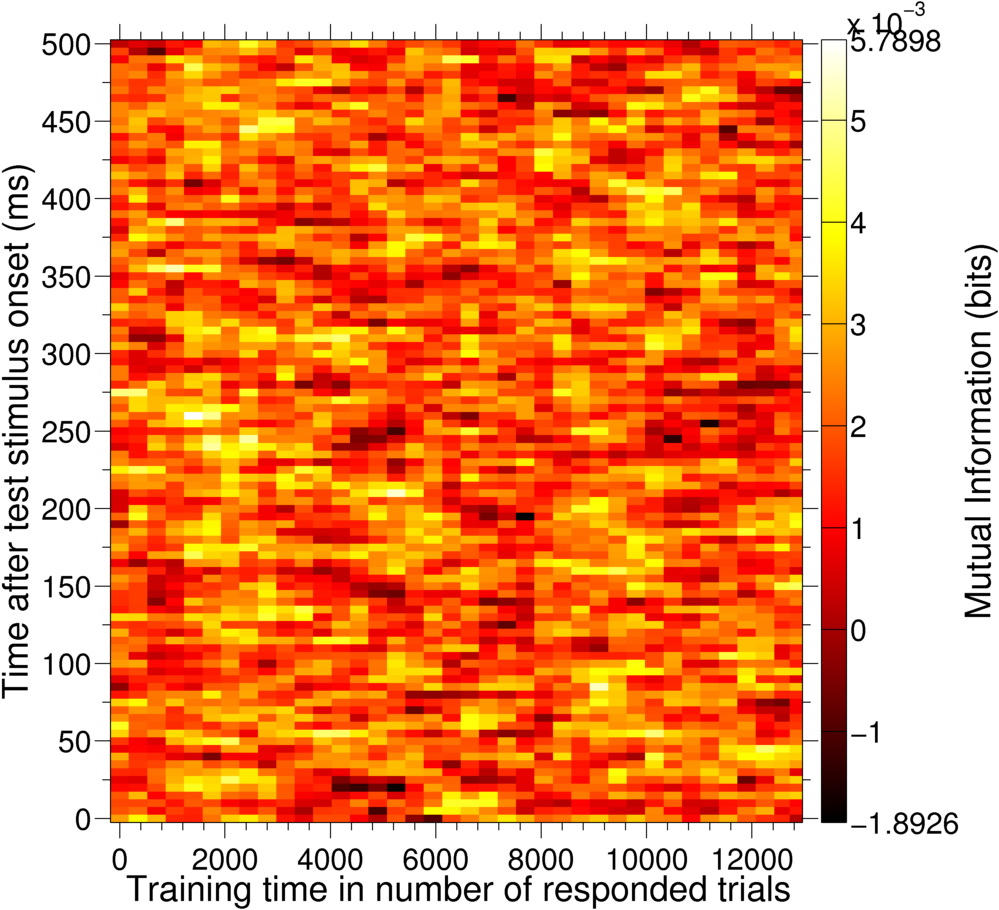
\includegraphics[scale=.25]{%
% % % figs/info/I_trialwise_blanco_v1_chmean23_s343-354,355.1,355.2,356-359_tp1_1bins_of_20ms_dr_pt_oc0_test_tc5-5-20,22-3-28,32,35-5-50,60,90_nt1400_ts350_rmvet1_rmvms0_pcolorhot_20120815T234326.png}
% % %         \caption{}
% % %         \label{fig:b1-1x20tp1ma}
% % %     \end{subfigure}
% % %     \\
% %     \begin{subfigure}[b]{0.5\linewidth}
% %         \centering
% %         \caption{}
% %         \label{fig:b1-1x20tp4}
% %         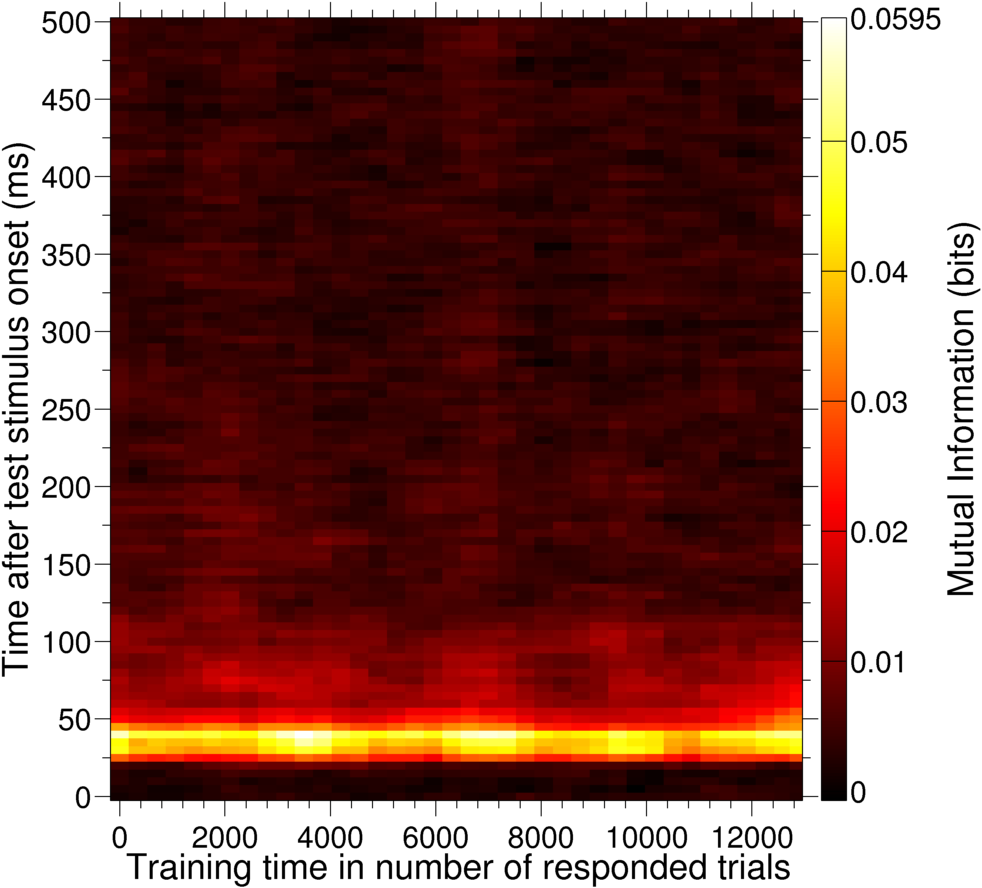
\includegraphics[scale=.25]{%
% % figs/info/I_trialwise_blanco_v1_chmean23_s343-354,355.1,355.2,356-359_tp4_1bins_of_20ms_dr_pt_oc0_test_tc5-5-20,22-3-28,32,35-5-50,60,90_nt1400_ts350_rmvet1_rmvms1_pcolorhot_20120815T234741.png}
% %     \end{subfigure}
% %     ~~
% %     \begin{subfigure}[b]{0.5\linewidth}
% %         \centering
% %         \caption{}
% %         \label{fig:b1-1x20tp1}
% %         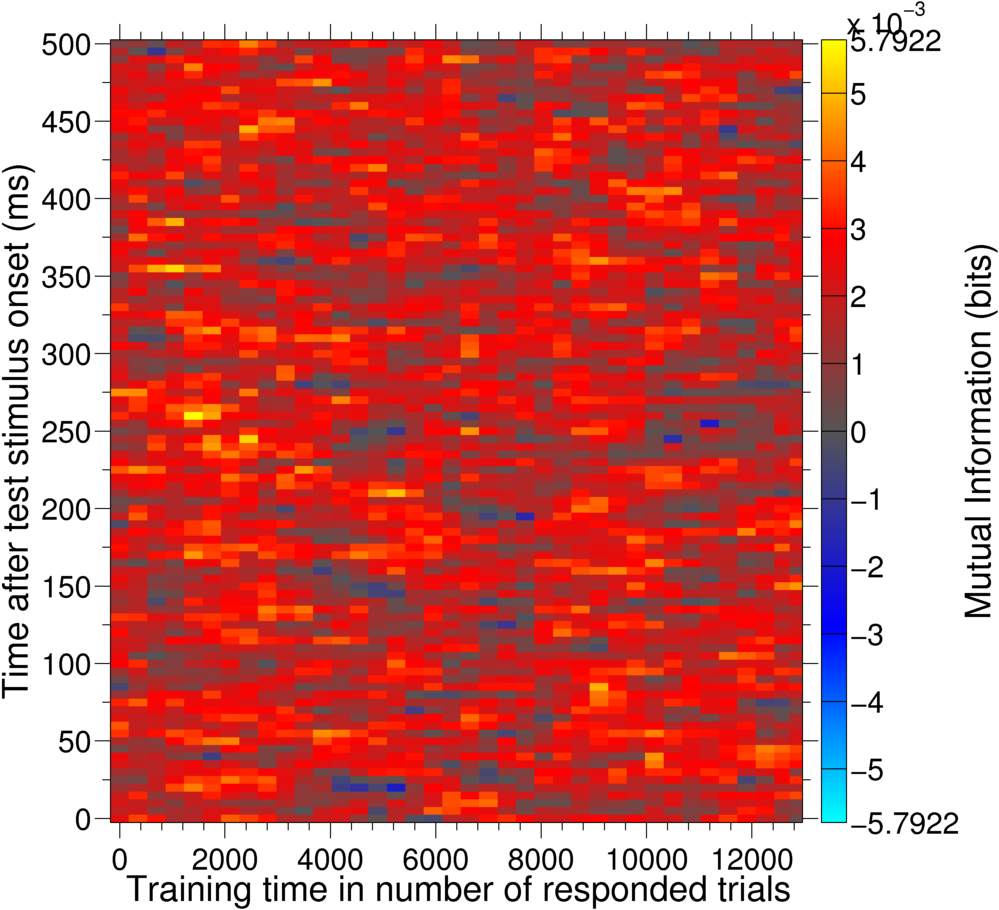
\includegraphics[scale=.25]{%
% % figs/info/I_trialwise_blanco_v1_chmean23_s343-354,355.1,355.2,356-359_tp1_1bins_of_20ms_dr_pt_oc0_test_tc5-5-20,22-3-28,32,35-5-50,60,90_nt1400_ts350_rmvet1_rmvms1_pcolorbp_20120816T175451.png}
% %     \end{subfigure}
% %     \\
% %     \begin{subfigure}[b]{0.5\linewidth}
% %         \centering
% %         \caption{}
% %         \label{fig:b1-5x4tp4}
% %         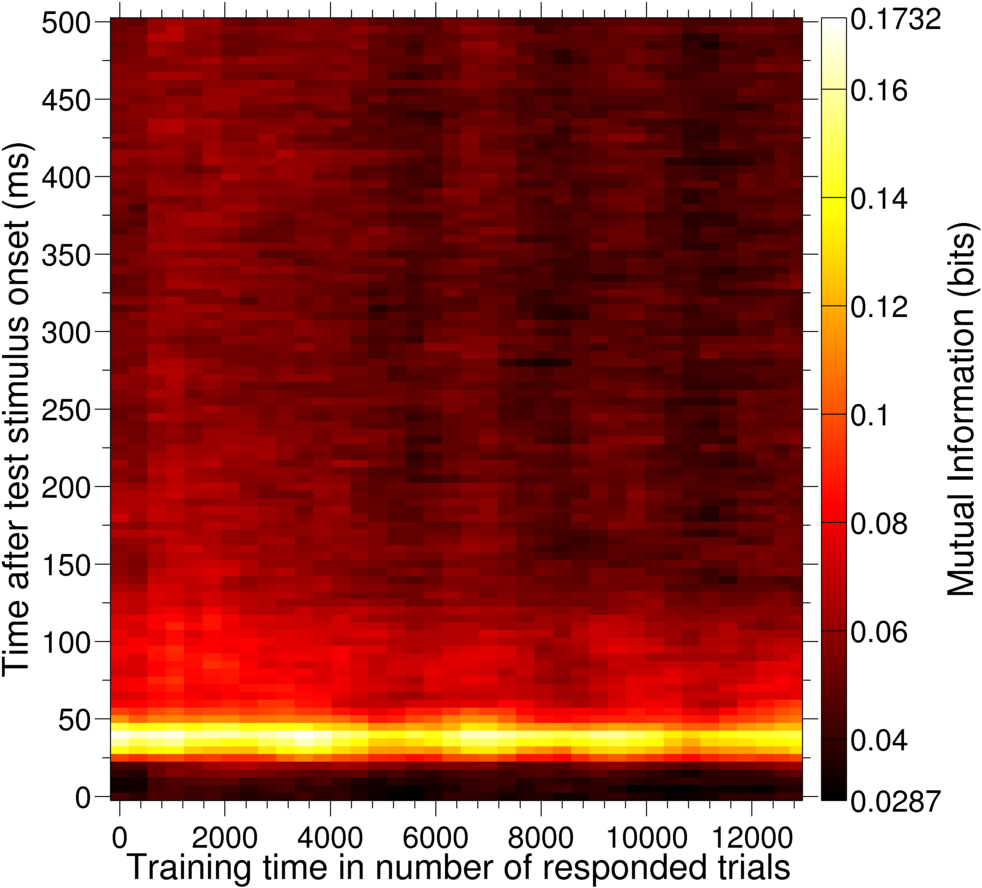
\includegraphics[scale=.25]{%
% % figs/info/I_trialwise_blanco_v1_chmean23_s343-354,355.1,355.2,356-359_tp4_5bins_of_4ms_dr_pt_oc0_test_tc5-5-20,22-3-28,32,35-5-50,60,90_nt1400_ts350_rmvet1_rmvms1_pcolorhot_20120815T234513.png}
% %     \end{subfigure}
% %     ~~
% %     \begin{subfigure}[b]{0.5\linewidth}
% %         \centering
% %         \caption{}
% %         \label{fig:b1-5x4tp1}
% %         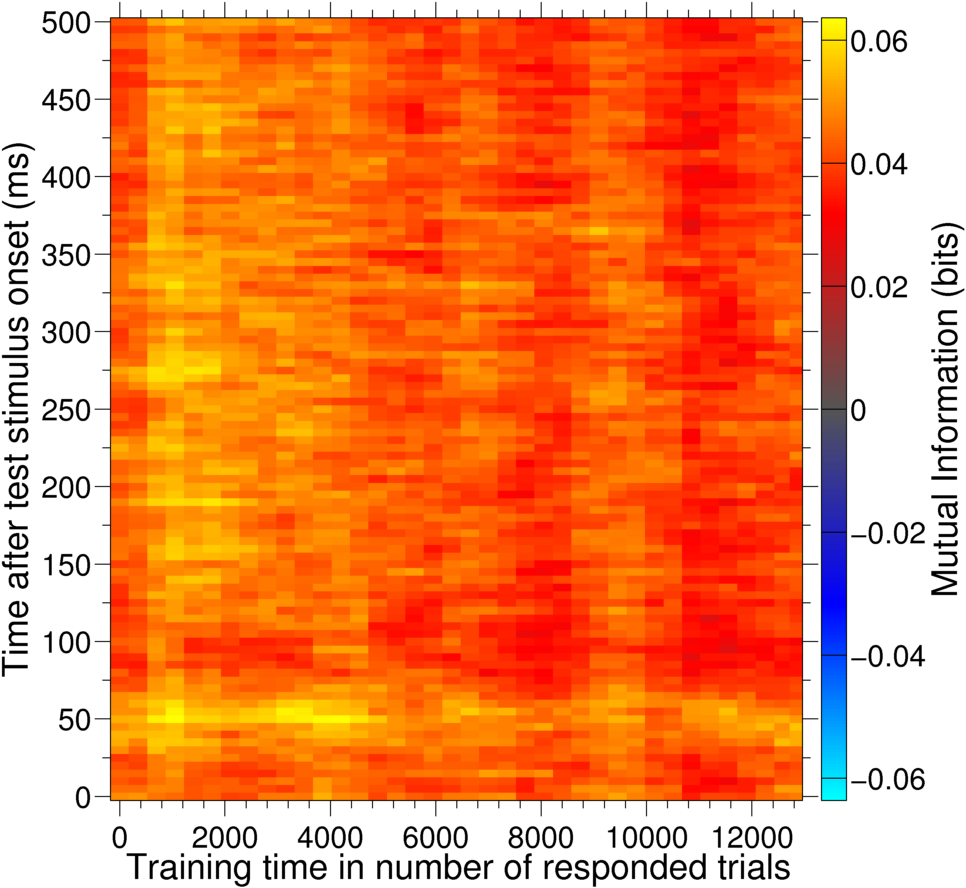
\includegraphics[scale=.25]{%
% % figs/info/I_trialwise_blanco_v1_chmean23_s343-354,355.1,355.2,356-359_tp1_5bins_of_4ms_dr_pt_oc0_test_tc5-5-20,22-3-28,32,35-5-50,60,90_nt1400_ts350_rmvet1_rmvms1_pcolorbp_20120816T175423.png}
% %     \end{subfigure}
% %     \caption{\ac{M1} \ac{V1}: Mutual information between the test stimulus and \SI{20}{ms} of spiking activity, averaged across 23 channels.
% % The \ac{PT} bias correction method was used in all estimates of the information, and the modification to the spiking data to remove the artifact as described in Sec.~\ref{sec:ma} was performed.
% % The neural code used in \ref{fig:b1-1x20tp4}, \ref{fig:b1-1x20tp1} is a spike count code, whilst in \ref{fig:b1-5x4tp4} and \ref{fig:b1-5x4tp1} it is a spike timing code where the \SI{20}{ms} window was subdivided into 5 bins each of \SI{4}{ms}.
% % In \ref{fig:b1-1x20tp4} and \ref{fig:b1-5x4tp4} the spike-train is taken from the test presentation part of the trial;
% % for \ref{fig:b1-1x20tp1} and \ref{fig:b1-5x4tp1} the spike-train is taken from spontaneous pre-stimulus activity.
% % The data is sampled in intervals of \SI{350}{trials} in the $x$-direction and \SI{5}{ms} in the $y$-direction, so there is significant correlation between any pair of pixels in the image with less than 4 pixels between them in either cartesian direction.
% % % In \ref{fig:b1-1x20tp4ma}, \ref{fig:b1-1x20tp4}, and \ref{fig:b1-5x4tp4}, the spike-train is taken from the test presentation part of the trial;
% % % for \ref{fig:b1-1x20tp1ma}, \ref{fig:b1-1x20tp1}, and \ref{fig:b1-5x4tp1}, the spike-train is taken from spontaneous pre-stimulus activity.
% % % In \ref{fig:b1-1x20tp4ma} and \ref{fig:b1-1x20tp1ma} no attempt was made to remove the monitor artifact from the raw data, whilst in the rest of the panels the data was modified to counter this as described in \ref{sec:ma}.
% % % \ref{fig:b1-1x20tp4ma}
% % % \ref{fig:b1-1x20tp1ma}
% % % \ref{fig:b1-1x20tp4}
% % % \ref{fig:b1-1x20tp1}
% % % \ref{fig:b1-5x4tp4}
% % % \ref{fig:b1-5x4tp1}
% % }
% %     \label{fig:b1-trialwise}
% % \end{figure}


% figs/info/I_trialwise_jack_v1_chmean25_s51-72_tp4_1bins_of_20ms_dr_pt_oc0_test_tc5-5-20,22-3-28,32,35-5-50,60,90_nt1400_ts350_rmvet1_rmvms0_pcolorhot_20120815T234410.png
% figs/info/I_trialwise_jack_v1_chmean25_s51-72_tp1_1bins_of_20ms_dr_pt_oc0_test_tc5-5-20,22-3-28,32,35-5-50,60,90_nt1400_ts350_rmvet1_rmvms0_pcolorhot_20120815T234245.png
% figs/info/I_trialwise_jack_v1_chmean25_s51-72_tp4_1bins_of_20ms_dr_pt_oc0_test_tc5-5-20,22-3-28,32,35-5-50,60,90_nt1400_ts350_rmvet1_rmvms1_pcolorhot_20120815T234701.png
% figs/info/I_trialwise_jack_v1_chmean25_s51-72_tp1_1bins_of_20ms_dr_pt_oc0_test_tc5-5-20,22-3-28,32,35-5-50,60,90_nt1400_ts350_rmvet1_rmvms1_pcolorbp_20120816T175411.png
% figs/info/I_trialwise_jack_v1_chmean25_s51-72_tp4_5bins_of_4ms_dr_pt_oc0_test_tc5-5-20,22-3-28,32,35-5-50,60,90_nt1400_ts350_rmvet1_rmvms1_pcolorhot_20120815T234434.png
% figs/info/I_trialwise_jack_v1_chmean25_s51-72_tp1_5bins_of_4ms_dr_pt_oc0_test_tc5-5-20,22-3-28,32,35-5-50,60,90_nt1400_ts350_rmvet1_rmvms1_pcolorbp_20120816T175343.png

% % \begin{figure}[htbp]
% % %     \begin{subfigure}[b]{0.5\linewidth}
% % %         \centering
% % %         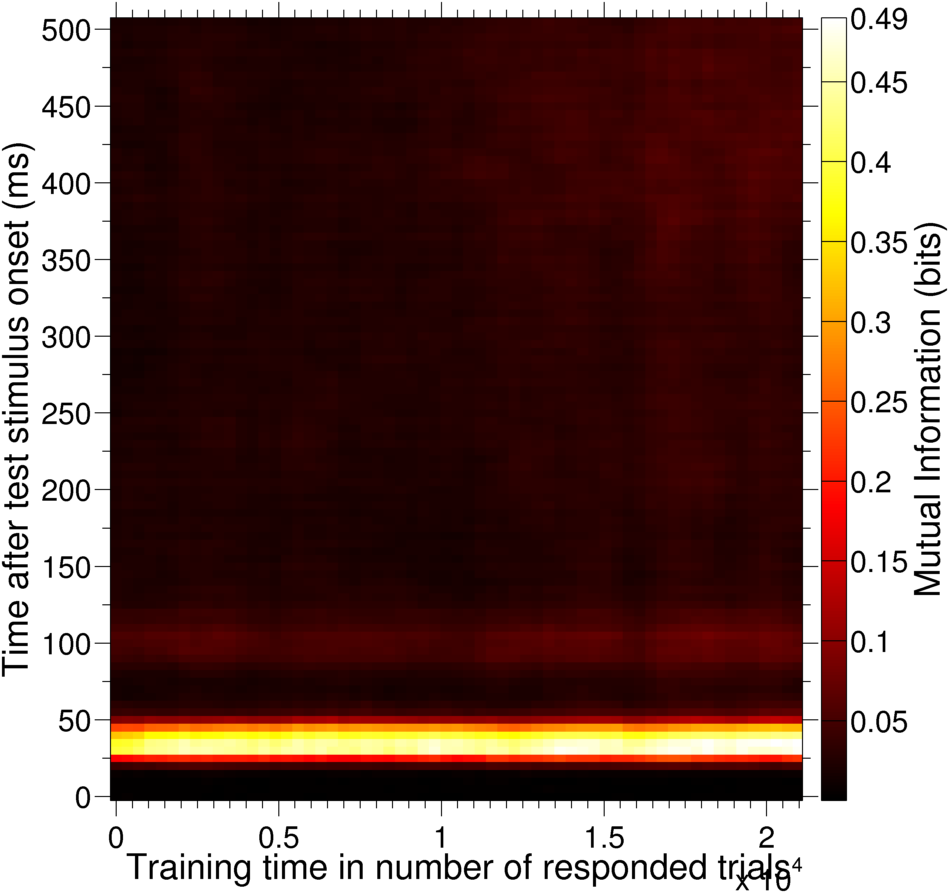
\includegraphics[scale=.25]{%
% % % figs/info/I_trialwise_jack_v1_chmean25_s51-72_tp4_1bins_of_20ms_dr_pt_oc0_test_tc5-5-20,22-3-28,32,35-5-50,60,90_nt1400_ts350_rmvet1_rmvms0_pcolorhot_20120815T234410.png}
% % %         \caption{}
% % %         \label{fig:j1-1x20tp4ma}
% % %     \end{subfigure}
% % %     ~~
% % %     \begin{subfigure}[b]{0.5\linewidth}
% % %         \centering
% % %         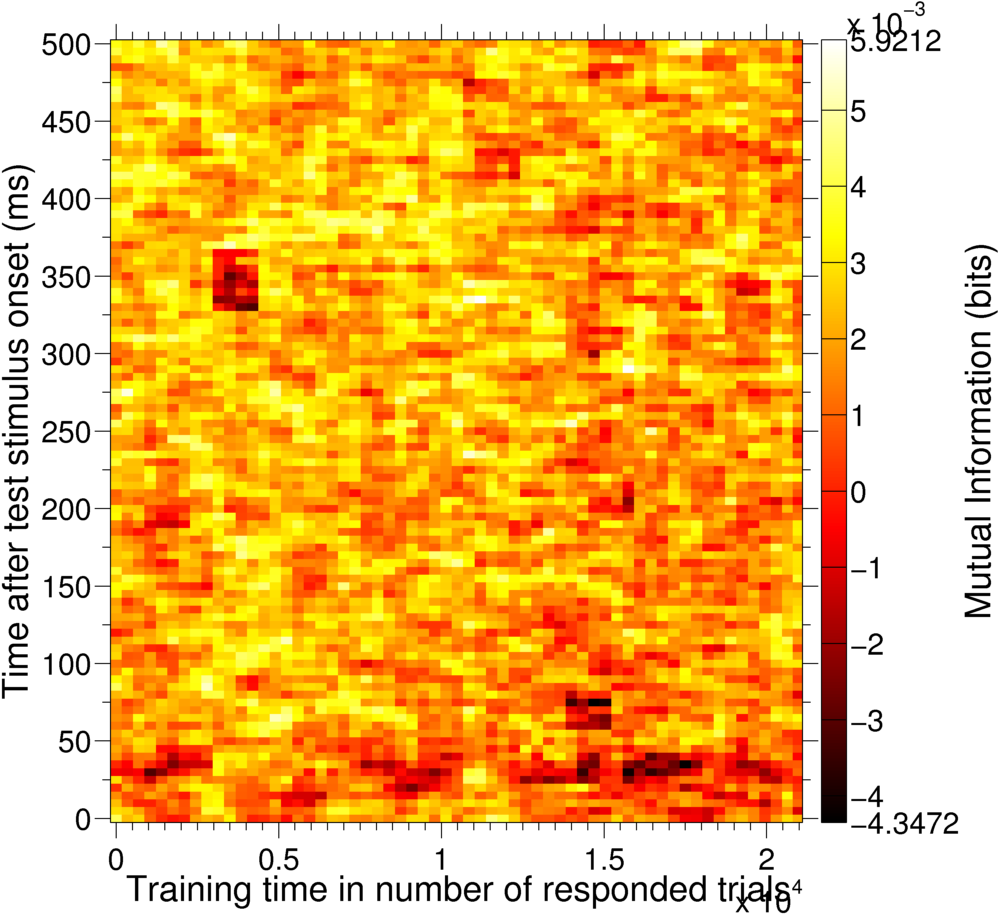
\includegraphics[scale=.25]{%
% % % figs/info/I_trialwise_jack_v1_chmean25_s51-72_tp1_1bins_of_20ms_dr_pt_oc0_test_tc5-5-20,22-3-28,32,35-5-50,60,90_nt1400_ts350_rmvet1_rmvms0_pcolorhot_20120815T234245.png}
% % %         \caption{}
% % %         \label{fig:j1-1x20tp1ma}
% % %     \end{subfigure}
% % %     \\
% %     \begin{subfigure}[b]{0.5\linewidth}
% %         \centering
% %         \caption{}
% %         \label{fig:j1-1x20tp4}
% %         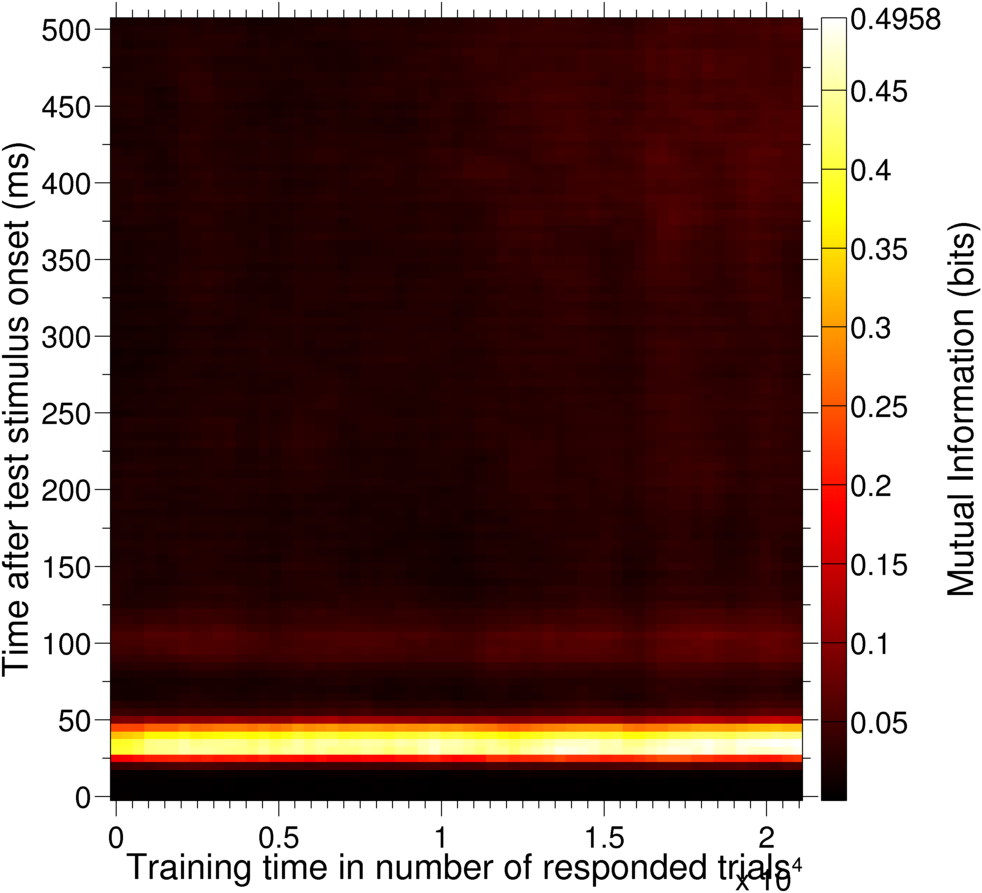
\includegraphics[scale=.25]{%
% % figs/info/I_trialwise_jack_v1_chmean25_s51-72_tp4_1bins_of_20ms_dr_pt_oc0_test_tc5-5-20,22-3-28,32,35-5-50,60,90_nt1400_ts350_rmvet1_rmvms1_pcolorhot_20120815T234701.png}
% %     \end{subfigure}
% %     ~~
% %     \begin{subfigure}[b]{0.5\linewidth}
% %         \centering
% %         \caption{}
% %         \label{fig:j1-1x20tp1}
% %         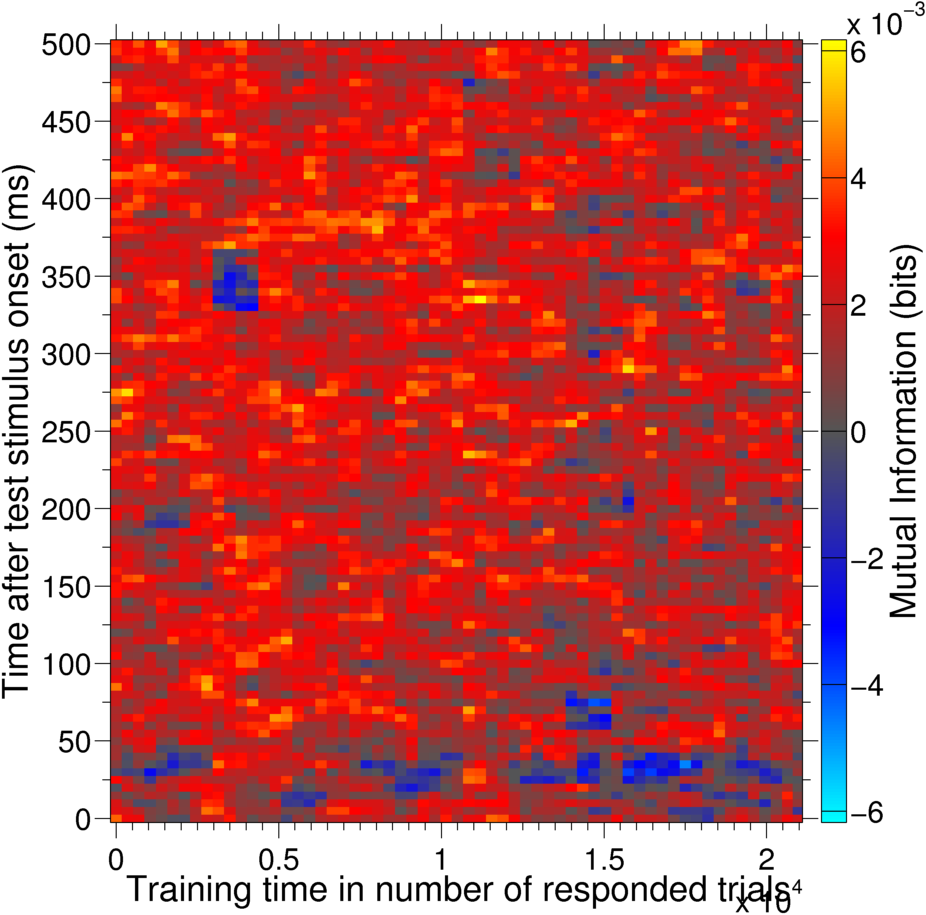
\includegraphics[scale=.25]{%
% % figs/info/I_trialwise_jack_v1_chmean25_s51-72_tp1_1bins_of_20ms_dr_pt_oc0_test_tc5-5-20,22-3-28,32,35-5-50,60,90_nt1400_ts350_rmvet1_rmvms1_pcolorbp_20120816T175411.png}
% %     \end{subfigure}
% %     \\
% %     \begin{subfigure}[b]{0.5\linewidth}
% %         \centering
% %         \caption{}
% %         \label{fig:j1-5x4tp4}
% %         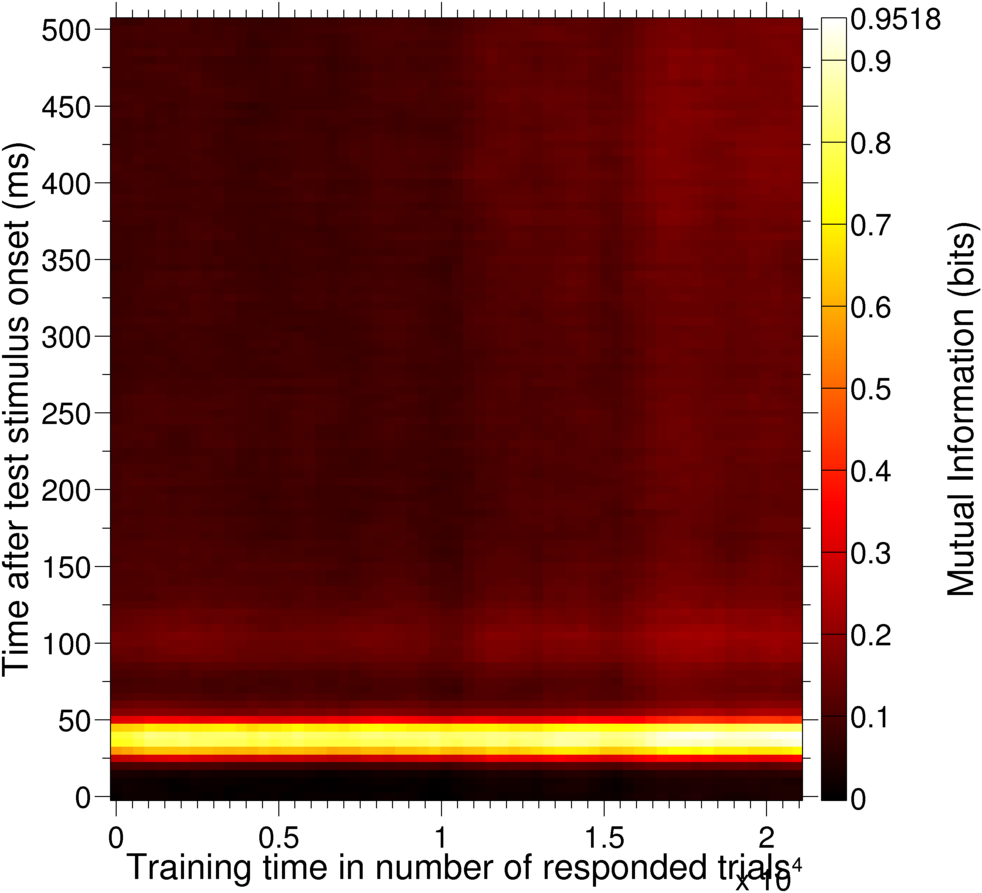
\includegraphics[scale=.25]{%
% % figs/info/I_trialwise_jack_v1_chmean25_s51-72_tp4_5bins_of_4ms_dr_pt_oc0_test_tc5-5-20,22-3-28,32,35-5-50,60,90_nt1400_ts350_rmvet1_rmvms1_pcolorhot_20120815T234434.png}
% %     \end{subfigure}
% %     ~~
% %     \begin{subfigure}[b]{0.5\linewidth}
% %         \centering
% %         \caption{}
% %         \label{fig:j1-5x4tp1}
% %         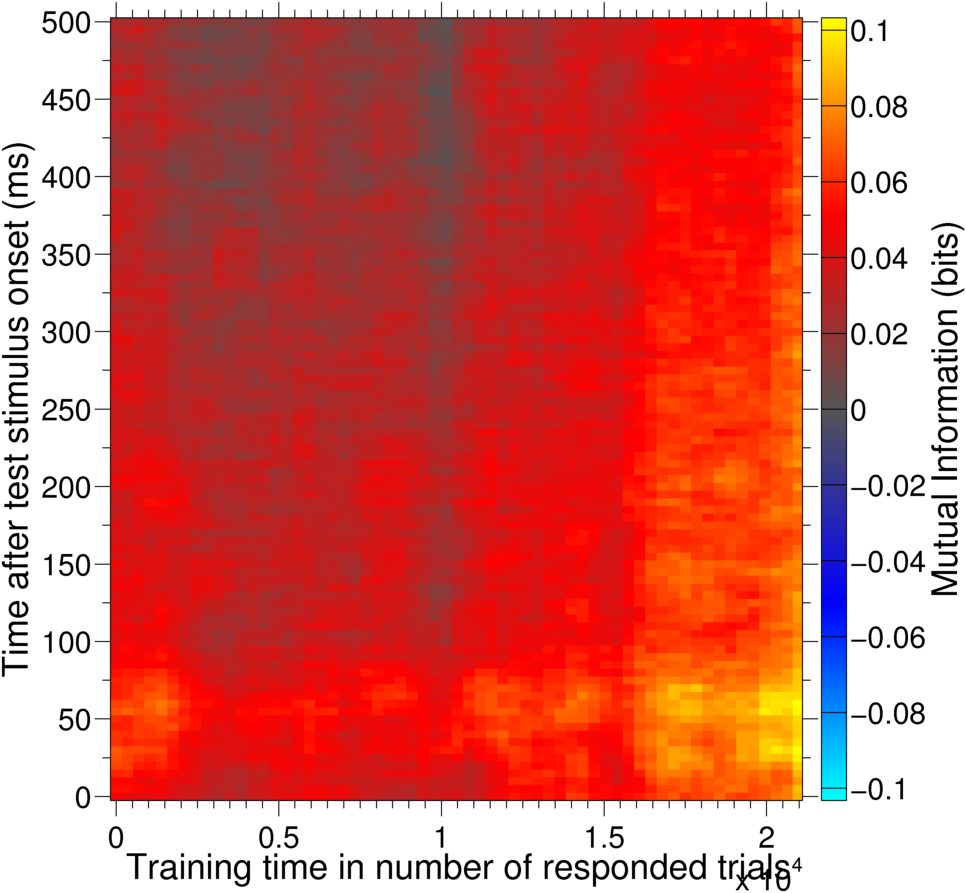
\includegraphics[scale=.25]{%
% % figs/info/I_trialwise_jack_v1_chmean25_s51-72_tp1_5bins_of_4ms_dr_pt_oc0_test_tc5-5-20,22-3-28,32,35-5-50,60,90_nt1400_ts350_rmvet1_rmvms1_pcolorbp_20120816T175343.png}
% %     \end{subfigure}
% %     \caption{\ac{M2} \ac{V1}: Mutual information between the test stimulus and \SI{20}{ms} of spiking activity, averaged across 25 channels.
% % The \ac{PT} bias correction method was used in all estimates of the information.
% % Panels \ref{fig:j1-1x20tp4}--\ref{fig:j1-5x4tp1} are the same as for Fig.~\ref{fig:b1-trialwise}.
% % % The neural code used in \ref{fig:j1-1x20tp4ma}--\ref{fig:j1-1x20tp1} is a spike count code, whilst in \ref{fig:j1-5x4tp4}, \ref{fig:j1-5x4tp1} it is a spike timing code where the \SI{20}{ms} window was subdivided into 5 bins each of \SI{4}{ms}.
% % % In \ref{fig:j1-1x20tp4ma}, \ref{fig:j1-1x20tp4}, and \ref{fig:j1-5x4tp4}, the spike-train is taken from the test presentation part of the trial;
% % % for \ref{fig:j1-1x20tp1ma}, \ref{fig:j1-1x20tp1}, and \ref{fig:j1-5x4tp1}, the spike-train is taken from spontaneous pre-stimulus activity.
% % % In \ref{fig:j1-1x20tp4ma} and \ref{fig:j1-1x20tp1ma} no attempt was made to remove the monitor artifact from the raw data, whilst in the rest of the panels the data was modified to counter this as described in \ref{sec:ma}.
% % % \ref{fig:j1-1x20tp4ma}
% % % \ref{fig:j1-1x20tp1ma}
% % % \ref{fig:j1-1x20tp4}
% % % \ref{fig:j1-1x20tp1}
% % % \ref{fig:j1-5x4tp4}
% % % \ref{fig:j1-5x4tp1}
% % }
% %     \label{fig:j1-trialwise}
% % \end{figure}

% figs/info/I_trialwise_blanco_v4_chmean31_s307,308,311,313,314,317,318,320,321,329-341_tp4_1bins_of_20ms_dr_pt_oc0_test_tc10-5-25,27-29,31-33,35,40-10-60_nt1400_ts350_rmvet1_rmvms0_pcolorhot_20120815T234508.png
% figs/info/I_trialwise_blanco_v4_chmean31_s307,308,311,313,314,317,318,320,321,329-341_tp1_1bins_of_20ms_dr_pt_oc0_test_tc10-5-25,27-29,31-33,35,40-10-60_nt1400_ts350_rmvet1_rmvms0_pcolorhot_20120815T234341.png
% figs/info/I_trialwise_blanco_v4_chmean31_s307,308,311,313,314,317,318,320,321,329-341_tp4_1bins_of_20ms_dr_pt_oc0_test_tc10-5-25,27-29,31-33,35,40-10-60_nt1400_ts350_rmvet1_rmvms1_pcolorhot_20120815T234756.png
% figs/info/I_trialwise_blanco_v4_chmean31_s307,308,311,313,314,317,318,320,321,329-341_tp1_1bins_of_20ms_dr_pt_oc0_test_tc10-5-25,27-29,31-33,35,40-10-60_nt1400_ts350_rmvet1_rmvms1_pcolorbp_20120816T175507.png
% figs/info/I_trialwise_blanco_v4_chmean31_s307,308,311,313,314,317,318,320,321,329-341_tp4_5bins_of_4ms_dr_pt_oc0_test_tc10-5-25,27-29,31-33,35,40-10-60_nt1400_ts350_rmvet1_rmvms1_pcolorhot_20120815T234528.png
% figs/info/I_trialwise_blanco_v4_chmean31_s307,308,311,313,314,317,318,320,321,329-341_tp1_5bins_of_4ms_dr_pt_oc0_test_tc10-5-25,27-29,31-33,35,40-10-60_nt1400_ts350_rmvet1_rmvms1_pcolorbp_20120816T175438.png

% % \cleartoevenpage

% % \begin{figure}[htbp]
% % %     \begin{subfigure}[b]{0.5\linewidth}
% % %         \centering
% % %         \includegraphics[scale=.25]{%
% % % figs/info/I_trialwise_blanco_v4_chmean31_s307,308,311,313,314,317,318,320,321,329-341_tp4_1bins_of_20ms_dr_pt_oc0_test_tc10-5-25,27-29,31-33,35,40-10-60_nt1400_ts350_rmvet1_rmvms0_pcolorhot_20120815T234508.png}
% % %         \caption{}
% % %         \label{fig:b4-1x20tp4ma}
% % %     \end{subfigure}
% % %     ~~
% % %     \begin{subfigure}[b]{0.5\linewidth}
% % %         \centering
% % %         \includegraphics[scale=.25]{%
% % % figs/info/I_trialwise_blanco_v4_chmean31_s307,308,311,313,314,317,318,320,321,329-341_tp1_1bins_of_20ms_dr_pt_oc0_test_tc10-5-25,27-29,31-33,35,40-10-60_nt1400_ts350_rmvet1_rmvms0_pcolorhot_20120815T234341.png}
% % %         \caption{}
% % %         \label{fig:b4-1x20tp1ma}
% % %     \end{subfigure}
% % %     \\
% %     \begin{subfigure}[b]{0.5\linewidth}
% %         \centering
% %         \caption{}
% %         \label{fig:b4-1x20tp4}
% %         \includegraphics[scale=.25]{%
% % figs/info/I_trialwise_blanco_v4_chmean31_s307,308,311,313,314,317,318,320,321,329-341_tp4_1bins_of_20ms_dr_pt_oc0_test_tc10-5-25,27-29,31-33,35,40-10-60_nt1400_ts350_rmvet1_rmvms1_pcolorhot_20120815T234756.png}
% %     \end{subfigure}
% %     ~~
% %     \begin{subfigure}[b]{0.5\linewidth}
% %         \centering
% %         \caption{}
% %         \label{fig:b4-1x20tp1}
% %         \includegraphics[scale=.25]{%
% % figs/info/I_trialwise_blanco_v4_chmean31_s307,308,311,313,314,317,318,320,321,329-341_tp1_1bins_of_20ms_dr_pt_oc0_test_tc10-5-25,27-29,31-33,35,40-10-60_nt1400_ts350_rmvet1_rmvms1_pcolorbp_20120816T175507.png}
% %     \end{subfigure}
% %     \\
% %     \begin{subfigure}[b]{0.5\linewidth}
% %         \centering
% %         \caption{}
% %         \label{fig:b4-5x4tp4}
% %         \includegraphics[scale=.25]{%
% % figs/info/I_trialwise_blanco_v4_chmean31_s307,308,311,313,314,317,318,320,321,329-341_tp4_5bins_of_4ms_dr_pt_oc0_test_tc10-5-25,27-29,31-33,35,40-10-60_nt1400_ts350_rmvet1_rmvms1_pcolorhot_20120815T234528.png}
% %     \end{subfigure}
% %     ~~
% %     \begin{subfigure}[b]{0.5\linewidth}
% %         \centering
% %         \caption{}
% %         \label{fig:b4-5x4tp1}
% %         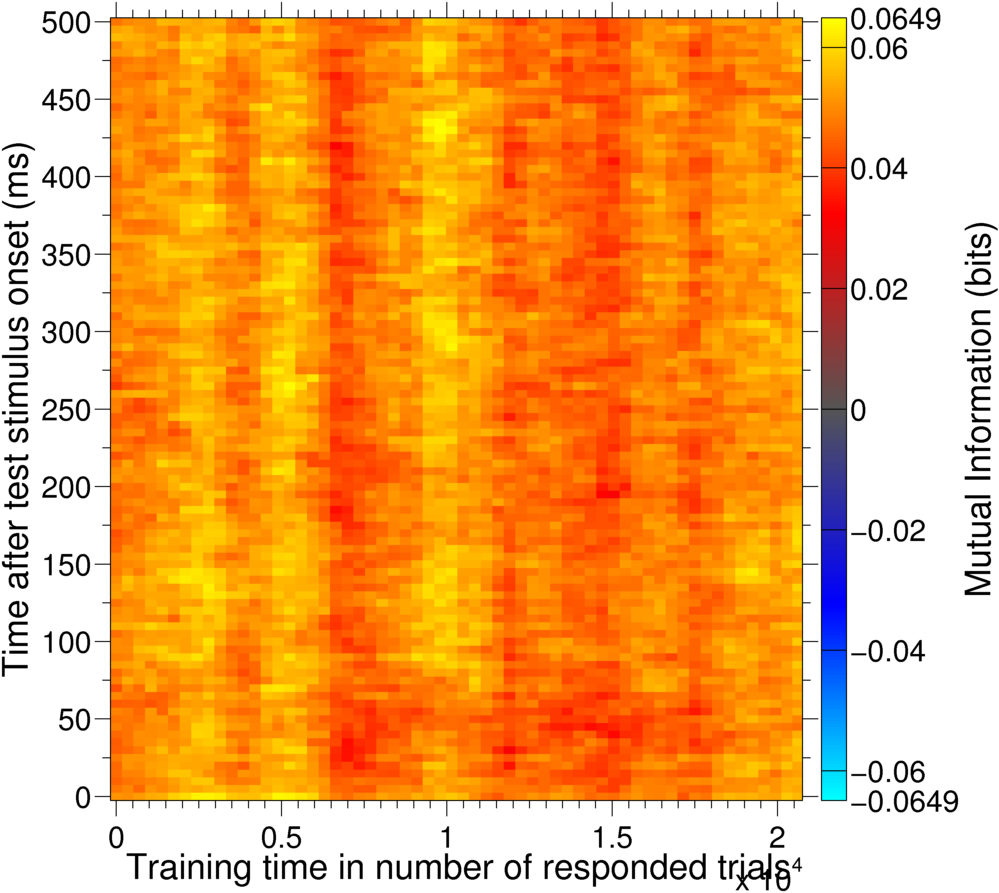
\includegraphics[scale=.25]{%
% % figs/info/I_trialwise_blanco_v4_chmean31_s307,308,311,313,314,317,318,320,321,329-341_tp1_5bins_of_4ms_dr_pt_oc0_test_tc10-5-25,27-29,31-33,35,40-10-60_nt1400_ts350_rmvet1_rmvms1_pcolorbp_20120816T175438.png}
% %     \end{subfigure}
% %     \caption{\ac{M1} \ac{V4}: Mutual information between the test stimulus and \SI{20}{ms} of spiking activity, averaged across 30 channels.
% % The \ac{PT} bias correction method was used in all estimates of the information.
% % Panels \ref{fig:b4-1x20tp4}--\ref{fig:b4-5x4tp1} are the same as for Fig.~\ref{fig:b1-trialwise}.
% % % The neural code used in \ref{fig:b4-1x20tp4ma}--\ref{fig:b4-1x20tp1} is a spike count code, whilst in \ref{fig:b4-5x4tp4}, \ref{fig:b4-5x4tp1} it is a spike timing code where the \SI{20}{ms} window was subdivided into 5 bins each of \SI{4}{ms}.
% % % In \ref{fig:b4-1x20tp4ma}, \ref{fig:b4-1x20tp4}, and \ref{fig:b4-5x4tp4}, the spike-train is taken from the test presentation part of the trial;
% % % for \ref{fig:b4-1x20tp1ma}, \ref{fig:b4-1x20tp1}, and \ref{fig:b4-5x4tp1}, the spike-train is taken from spontaneous pre-stimulus activity.
% % % In \ref{fig:b4-1x20tp4ma} and \ref{fig:b4-1x20tp1ma} no attempt was made to remove the monitor artifact from the raw data, whilst in the rest of the panels the data was modified to counter this as described in \ref{sec:ma}.
% % % \ref{fig:b4-1x20tp4ma}
% % % \ref{fig:b4-1x20tp1ma}
% % % \ref{fig:b4-1x20tp4}
% % % \ref{fig:b4-1x20tp1}
% % % \ref{fig:b4-5x4tp4}
% % % \ref{fig:b4-5x4tp1}
% % }
% %     \label{fig:b4-trialwise}
% % \end{figure}



% figs/info/I_trialwise_jack_v4_chmean20_s24-49_tp4_1bins_of_20ms_dr_pt_oc0_test_tc10-5-25,27-29,31-33,35,40-10-60_nt1400_ts350_rmvet1_rmvms0_pcolorhot_20120815T234433.png
% figs/info/I_trialwise_jack_v4_chmean20_s24-49_tp1_1bins_of_20ms_dr_pt_oc0_test_tc10-5-25,27-29,31-33,35,40-10-60_nt1400_ts350_rmvet1_rmvms1_pcolorbp_20120816T175433.png
% figs/info/I_trialwise_jack_v4_chmean20_s24-49_tp4_1bins_of_20ms_dr_pt_oc0_test_tc10-5-25,27-29,31-33,35,40-10-60_nt1400_ts350_rmvet1_rmvms1_pcolorhot_20120815T234723.png
% figs/info/I_trialwise_jack_v4_chmean20_s24-49_tp1_1bins_of_20ms_dr_pt_oc0_test_tc10-5-25,27-29,31-33,35,40-10-60_nt1400_ts350_rmvet1_rmvms1_pcolorhot_20120815T234559.png
% figs/info/I_trialwise_jack_v4_chmean20_s24-49_tp4_5bins_of_4ms_dr_pt_oc0_test_tc10-5-25,27-29,31-33,35,40-10-60_nt1400_ts350_rmvet1_rmvms1_pcolorhot_20120815T234455.png
% figs/info/I_trialwise_jack_v4_chmean20_s24-49_tp1_5bins_of_4ms_dr_pt_oc0_test_tc10-5-25,27-29,31-33,35,40-10-60_nt1400_ts350_rmvet1_rmvms1_pcolorbp_20120816T175404.png

% % \begin{figure}[htbp]
% % %     \begin{subfigure}[b]{0.5\linewidth}
% % %         \centering
% % %         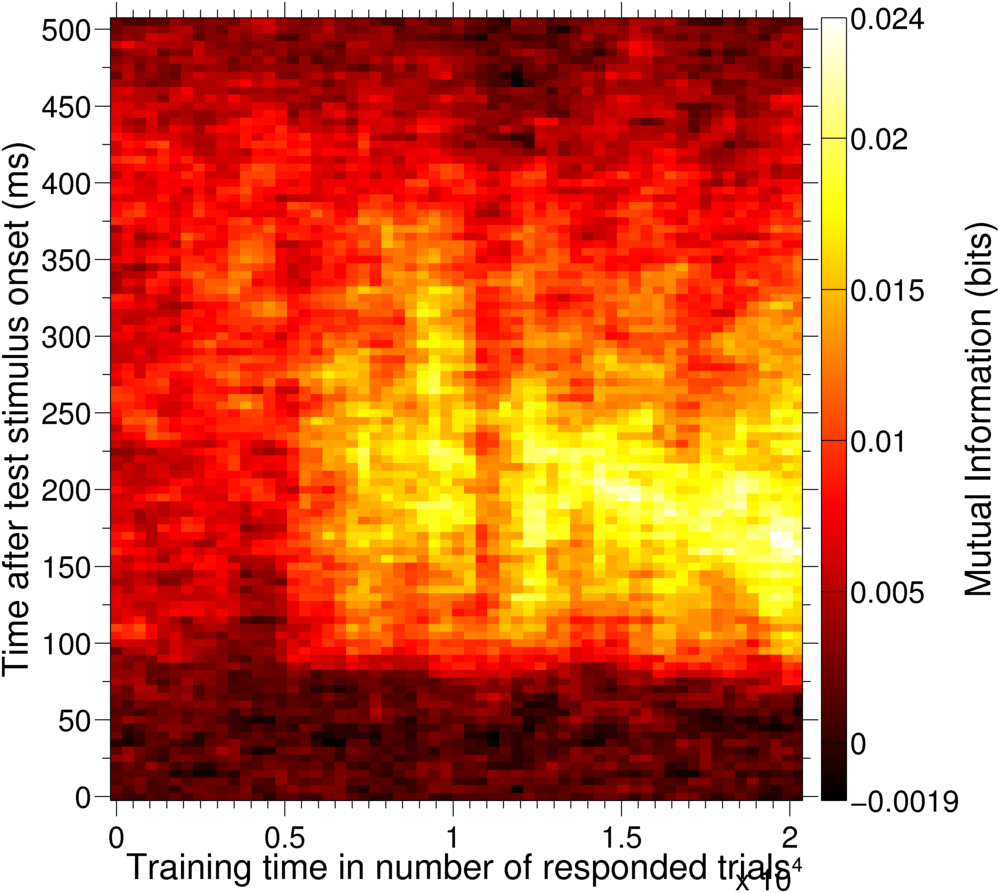
\includegraphics[scale=.25]{%
% % % figs/info/I_trialwise_jack_v4_chmean20_s24-49_tp4_1bins_of_20ms_dr_pt_oc0_test_tc10-5-25,27-29,31-33,35,40-10-60_nt1400_ts350_rmvet1_rmvms0_pcolorhot_20120815T234433.png}
% % %         \caption{}
% % %         \label{fig:j4-1x20tp4ma}
% % %     \end{subfigure}
% % %     ~~
% % %     \begin{subfigure}[b]{0.5\linewidth}
% % %         \centering
% % %         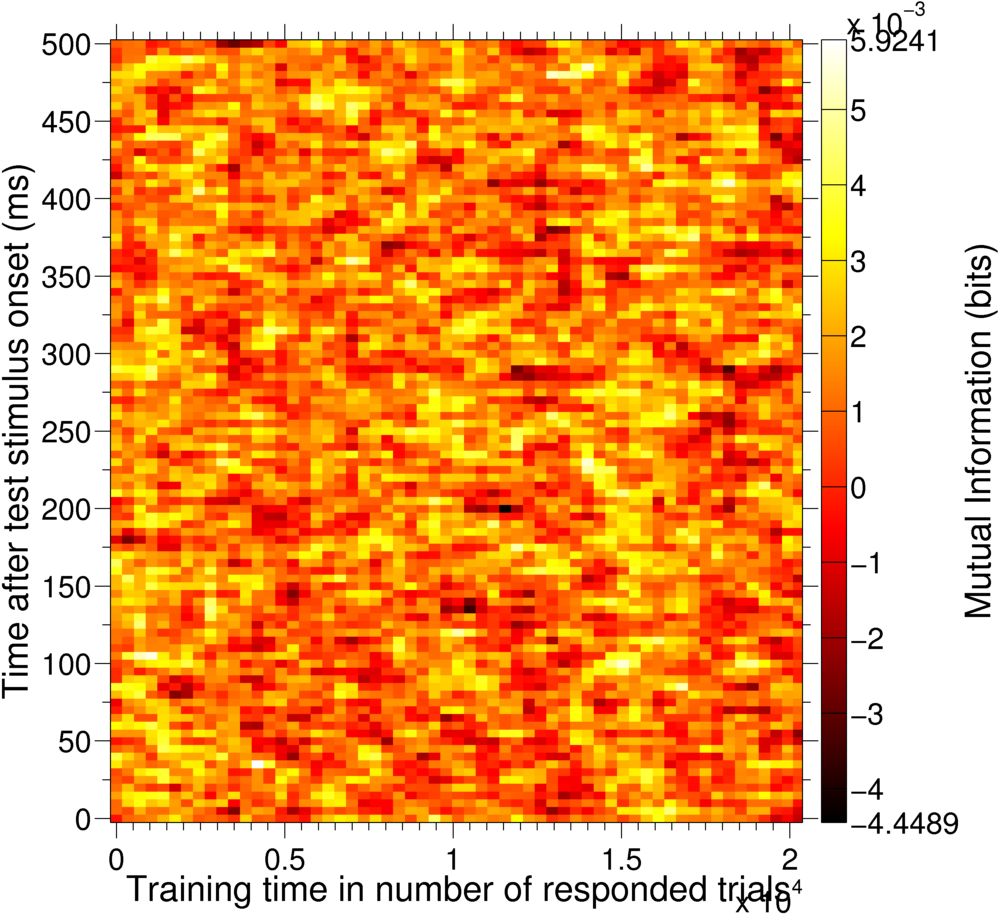
\includegraphics[scale=.25]{%
% % % figs/info/I_trialwise_jack_v4_chmean20_s24-49_tp1_1bins_of_20ms_dr_pt_oc0_test_tc10-5-25,27-29,31-33,35,40-10-60_nt1400_ts350_rmvet1_rmvms0_pcolorhot_20120815T234307.png}
% % %         \caption{}
% % %         \label{fig:j4-1x20tp1ma}
% % %     \end{subfigure}
% % %     \\
% %     \begin{subfigure}[b]{0.5\linewidth}
% %         \centering
% %         \caption{}
% %         \label{fig:j4-1x20tp4}
% %         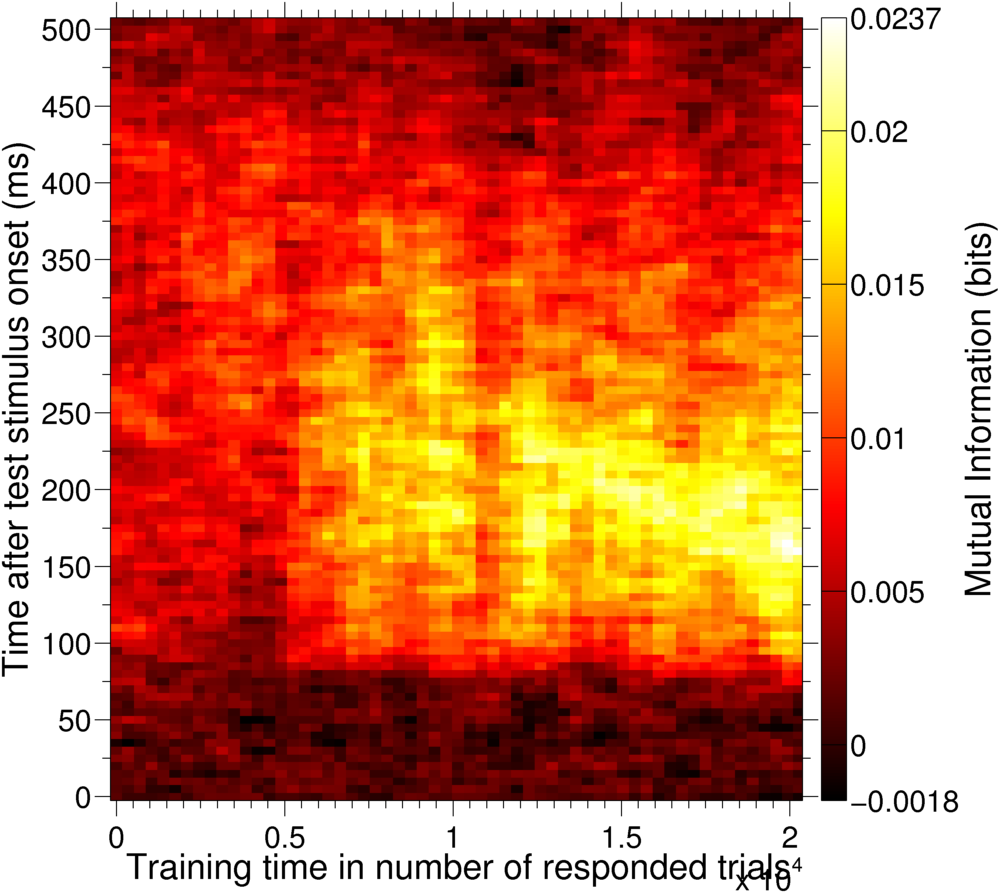
\includegraphics[scale=.25]{%
% % figs/info/I_trialwise_jack_v4_chmean20_s24-49_tp4_1bins_of_20ms_dr_pt_oc0_test_tc10-5-25,27-29,31-33,35,40-10-60_nt1400_ts350_rmvet1_rmvms1_pcolorhot_20120815T234723.png}
% %     \end{subfigure}
% %     ~~
% %     \begin{subfigure}[b]{0.5\linewidth}
% %         \centering
% %         \caption{}
% %         \label{fig:j4-1x20tp1}
% %         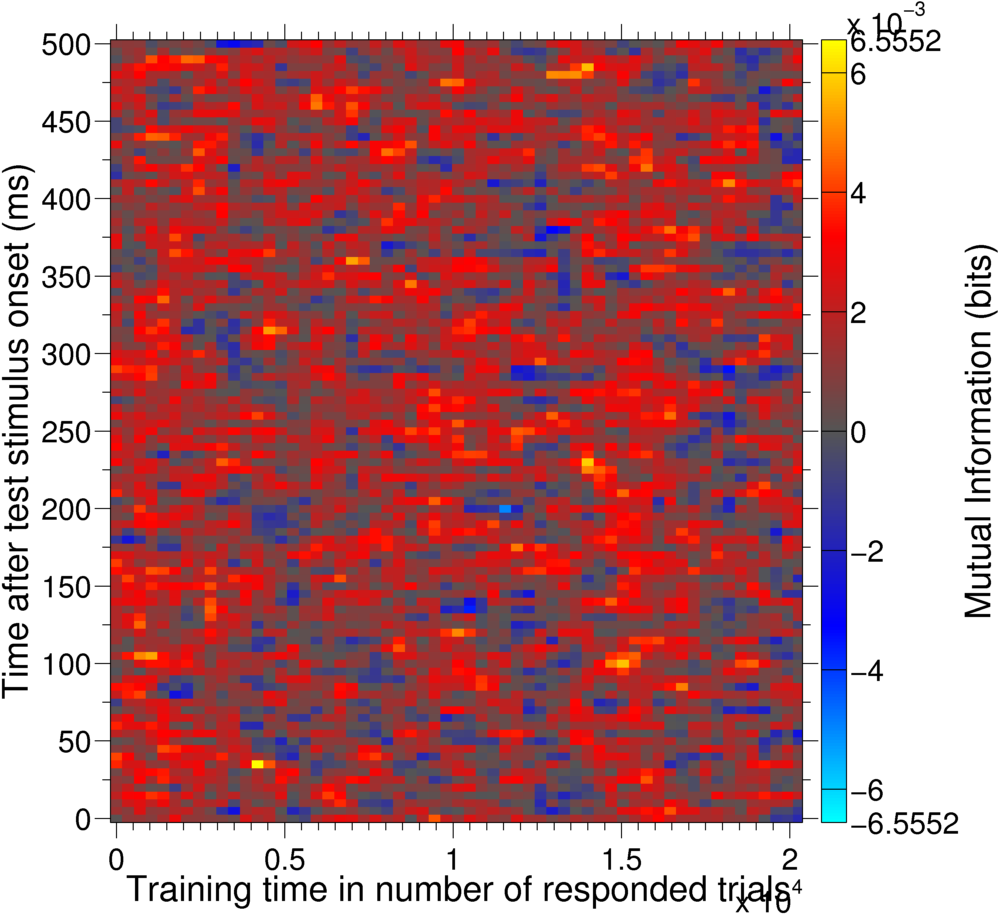
\includegraphics[scale=.25]{%
% % figs/info/I_trialwise_jack_v4_chmean20_s24-49_tp1_1bins_of_20ms_dr_pt_oc0_test_tc10-5-25,27-29,31-33,35,40-10-60_nt1400_ts350_rmvet1_rmvms1_pcolorbp_20120816T175433.png}
% %     \end{subfigure}
% %     \\
% %     \begin{subfigure}[b]{0.5\linewidth}
% %         \centering
% %         \caption{}
% %         \label{fig:j4-5x4tp4}
% %         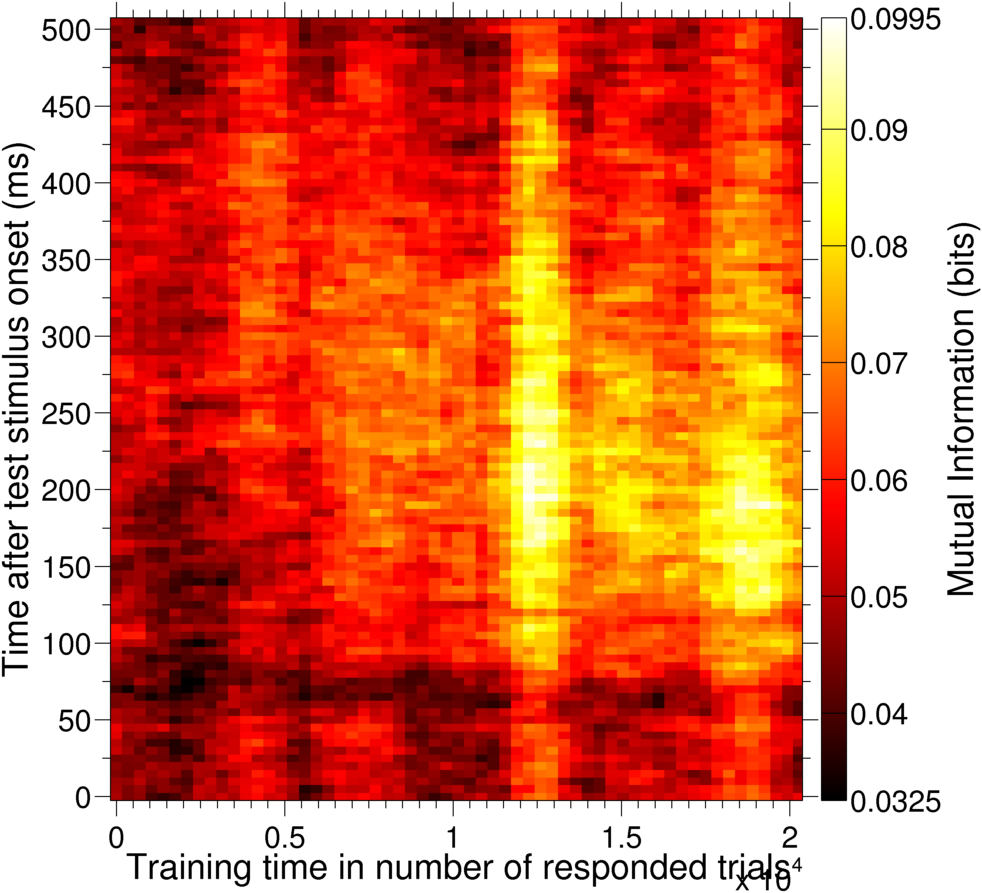
\includegraphics[scale=.25]{%
% % figs/info/I_trialwise_jack_v4_chmean20_s24-49_tp4_5bins_of_4ms_dr_pt_oc0_test_tc10-5-25,27-29,31-33,35,40-10-60_nt1400_ts350_rmvet1_rmvms1_pcolorhot_20120815T234455.png}
% %     \end{subfigure}
% %     ~~
% %     \begin{subfigure}[b]{0.5\linewidth}
% %         \centering
% %         \caption{}
% %         \label{fig:j4-5x4tp1}
% %         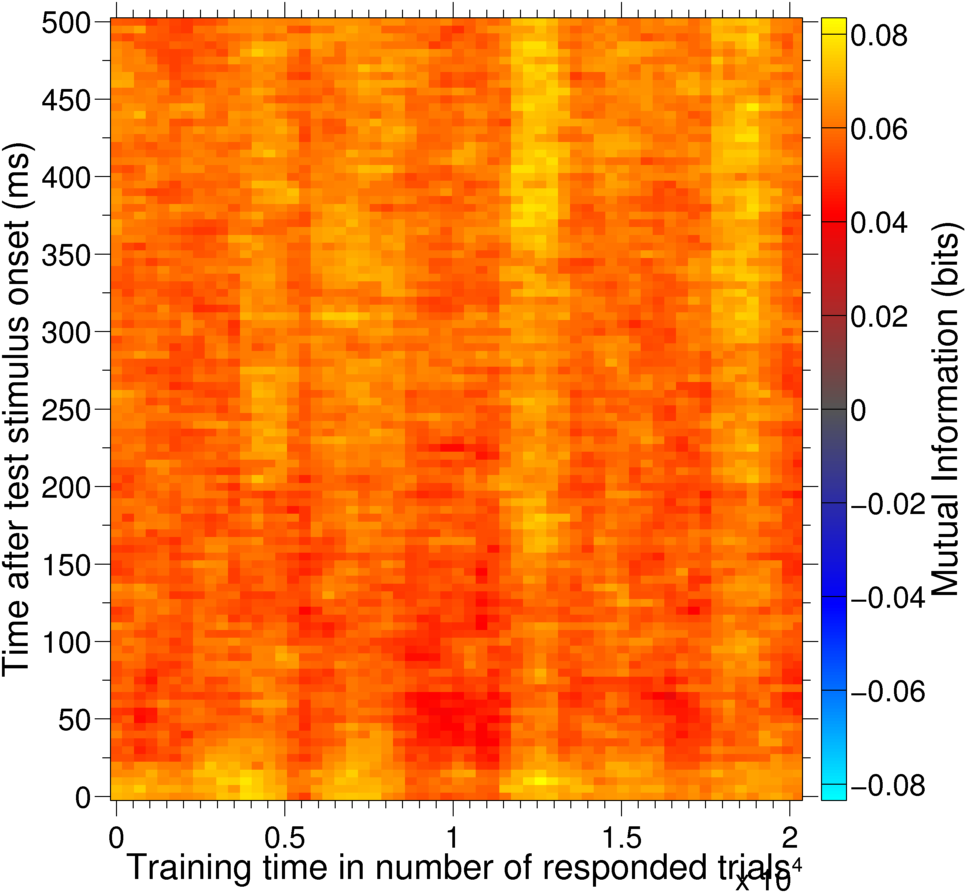
\includegraphics[scale=.25]{%
% % figs/info/I_trialwise_jack_v4_chmean20_s24-49_tp1_5bins_of_4ms_dr_pt_oc0_test_tc10-5-25,27-29,31-33,35,40-10-60_nt1400_ts350_rmvet1_rmvms1_pcolorbp_20120816T175404.png}
% %     \end{subfigure}
% %     \caption{\ac{M2} \ac{V4}: Mutual information between the test stimulus and \SI{20}{ms} of spiking activity, averaged across 20 channels.
% % The \ac{PT} bias correction method was used in all estimates of the information.
% % Panels \ref{fig:j4-1x20tp4}--\ref{fig:j4-5x4tp1} are the same as for Fig.~\ref{fig:b1-trialwise}.
% % % The neural code used in \ref{fig:j4-1x20tp4ma}--\ref{fig:j4-1x20tp1} is a spike count code, whilst in \ref{fig:j4-5x4tp4}, \ref{fig:j4-5x4tp1} it is a spike timing code where the \SI{20}{ms} window was subdivided into 5 bins each of \SI{4}{ms}.
% % % In \ref{fig:j4-1x20tp4ma}, \ref{fig:j4-1x20tp4}, and \ref{fig:j4-5x4tp4}, the spike-train is taken from the test presentation part of the trial;
% % % for \ref{fig:j4-1x20tp1ma}, \ref{fig:j4-1x20tp1}, and \ref{fig:j4-5x4tp1}, the spike-train is taken from spontaneous pre-stimulus activity.
% % % In \ref{fig:j4-1x20tp4ma} and \ref{fig:j4-1x20tp1ma} no attempt was made to remove the monitor artifact from the raw data, whilst in the rest of the panels the data was modified to counter this as described in \ref{sec:ma}.
% % % \ref{fig:j4-1x20tp4ma}
% % % \ref{fig:j4-1x20tp1ma}
% % % \ref{fig:j4-1x20tp4}
% % % \ref{fig:j4-1x20tp1}
% % % \ref{fig:j4-5x4tp4}
% % % \ref{fig:j4-5x4tp1}
% % }
% %     \label{fig:j4-trialwise}
% % \end{figure}

% 20, 30 and \SI{40}{ms} all tried.
% Mutual information increases as the duration increases as one would expect, but there is no other significant difference.
% Consequently only 20ms is shown in this section.

% More information with only correct trials used, but this could be due to differences in $P(S)$.

Turning our attention to the \ac{V4} results in Figs.~\ref{fig:b4-trialwise} and \ref{fig:j4-trialwise}, we can see the effect of the transient is present in \ac{M1}'s data (at the later start time of \SI{75}{ms}), but not in \ac{M2}'s.
This is surprising because, looking at the rasters, in both animals there are some channels which exhibit a transient response and some which do not.

Similar to \ac{V1}, it seems as if there is four times as much information in the timebinned code compared with the count code.
However, there is much more information measured for the spontaneous activity data again.
This is not reduced by increasing the number of trials either.

For the spike count code in \ac{M2}, the spontaneous information is nearly distributed around 0, suggesting the bias has been all but removed and the data is of very high quality.
For this animal, we can see a distinct increase in the information content with time, for both the spike count and timing codes.
Simultaneously, there is a movement of the peak information to earlier times closer to the stimulus onset.

In \ac{M1}, there is a small increase in the information content with time which may or may not significant.
However, it is reassuring to see that this is not due to an improvement in the data with time, as the trend in the spontaneous activity information bias (Fig.~\ref{fig:j4-5x4tp1}) is a decrease with time.

%------------------------------------------------------------------------------
\FloatBarrier
\subsection{Fine vs coarse contrast differences}

Comparing Figs.~\ref{fig:b1-1x20cc} and \ref{fig:j1-1x20cc} where the outer 6 contrasts are included with Figs.~\ref{fig:b1-1x20tp4} and \ref{fig:b1-1x20tp4} where all contrasts are included, it seems as if the amount of information has increased, which should not be possible.
However, the difference will be due to the difference in trials contained in each of the analyses.
In each case, an average of 100 trials per stimulus is used, but since the easier test conditions are presented less frequently, they are under-represented in Figs.~\ref{fig:b1-1x20tp4} and \ref{fig:b1-1x20tp4} (about 75 trials per stimulus).
Obviously these are more discriminable, so the under-representation comparably reduces the information.

Looking at \ac{V1} (Fig.~\ref{fig:v1-fvc}), we observe there is much more information for \ac{M2} than \ac{M1}, as we found before.
The quality of the data seems to have severely hampered the analysis for \ac{M1}, destroying the the fine differences in the data needed to evaluate the information contained about fine contrast differences (Fig.~\ref{fig:b1-1x20fc}).

Unsurprisingly, there is more information when considering the coarsely distinct contrasts than the finer differences, as the neural activity is bound to be more discriminable for these.
For \ac{M2}, there is a small upward trend again for both coarse and fine contrast differences, which may or may not be genuine.

% figs/info/I_trialwise_blanco_v1_chmean23_s343-354,355.1,355.2,356-359_tp4_1bins_of_20ms_dr_pt_oc0_test_tc5,15,22,40,50,90_nt600_ts150_rmvet1_rmvms1_pcolorhot_20120816T011936.png
% figs/info/I_trialwise_blanco_v1_chmean23_s343-354,355.1,355.2,356-359_tp4_1bins_of_20ms_dr_pt_oc0_test_tc22-3-28,32,35,40_nt600_ts150_rmvet1_rmvms1_pcolorhot_20120816T011920.png
% figs/info/I_trialwise_jack_v1_chmean25_s51-72_tp4_1bins_of_20ms_dr_pt_oc0_test_tc5,15,22,40,50,90_nt600_ts150_rmvet1_rmvms1_pcolorhot_20120816T011822.png
% figs/info/I_trialwise_jack_v1_chmean25_s51-72_tp4_1bins_of_20ms_dr_pt_oc0_test_tc22-3-28,32,35,40_nt600_ts150_rmvet1_rmvms1_pcolorhot_20120816T011800.png

% % \begin{figure}[htbp]
% %     \begin{subfigure}[b]{0.5\linewidth}
% %         \centering
% %         \caption{}
% %         \label{fig:b1-1x20cc}
% %         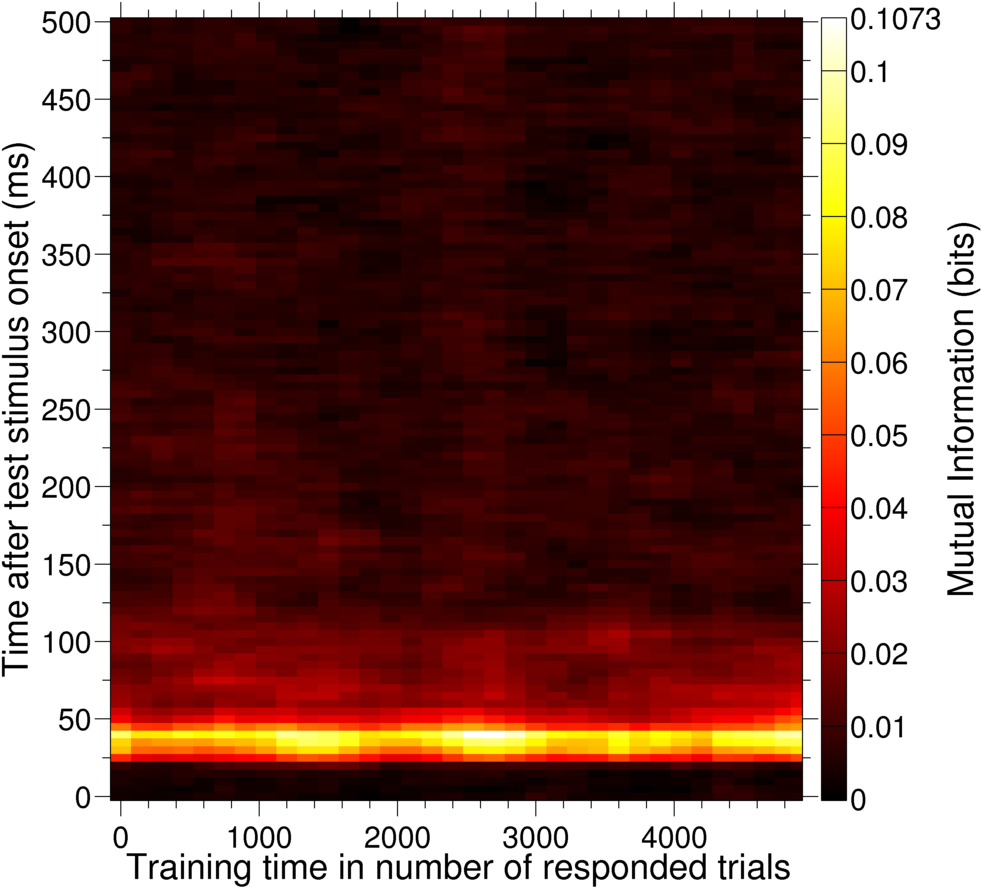
\includegraphics[scale=.25]{%
% % figs/info/I_trialwise_blanco_v1_chmean23_s343-354,355.1,355.2,356-359_tp4_1bins_of_20ms_dr_pt_oc0_test_tc5,15,22,40,50,90_nt600_ts150_rmvet1_rmvms1_pcolorhot_20120816T011936.png}
% %     \end{subfigure}
% %     ~~
% %     \begin{subfigure}[b]{0.5\linewidth}
% %         \centering
% %         \caption{}
% %         \label{fig:j1-1x20cc}
% %         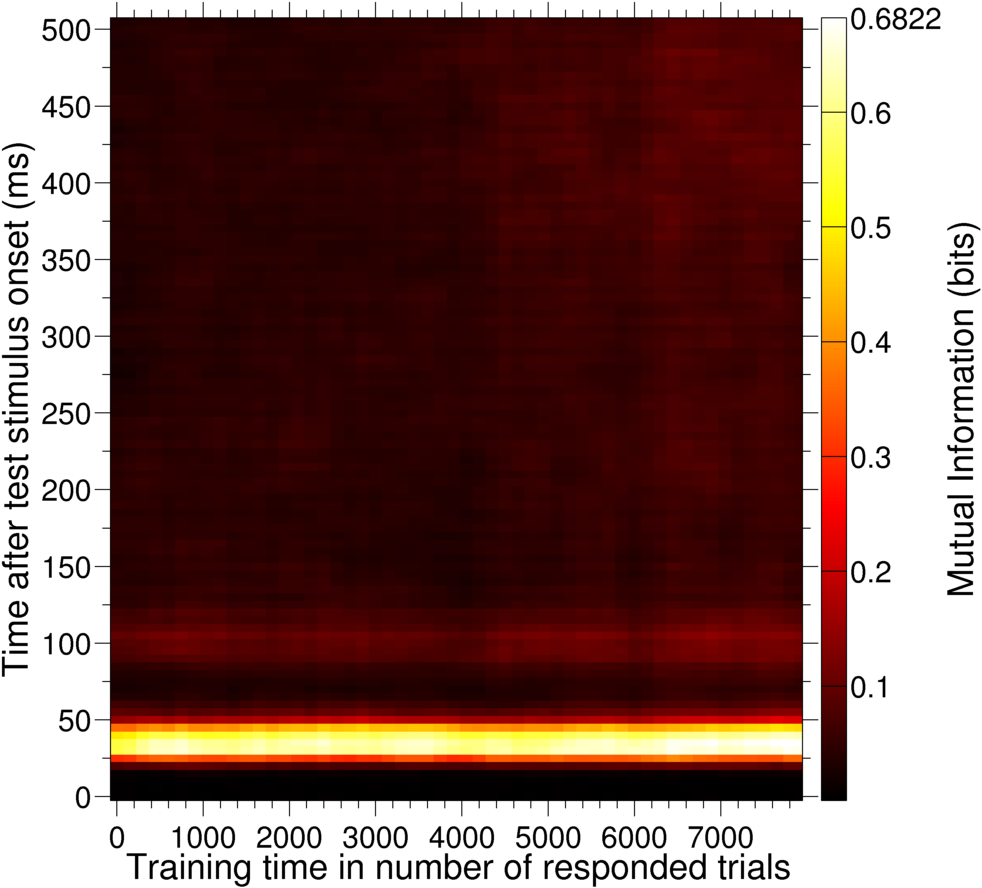
\includegraphics[scale=.25]{%
% % figs/info/I_trialwise_jack_v1_chmean25_s51-72_tp4_1bins_of_20ms_dr_pt_oc0_test_tc5,15,22,40,50,90_nt600_ts150_rmvet1_rmvms1_pcolorhot_20120816T011822.png}
% %     \end{subfigure}
% %     \\
% %     \begin{subfigure}[b]{0.5\linewidth}
% %         \centering
% %         \caption{}
% %         \label{fig:b1-1x20fc}
% %         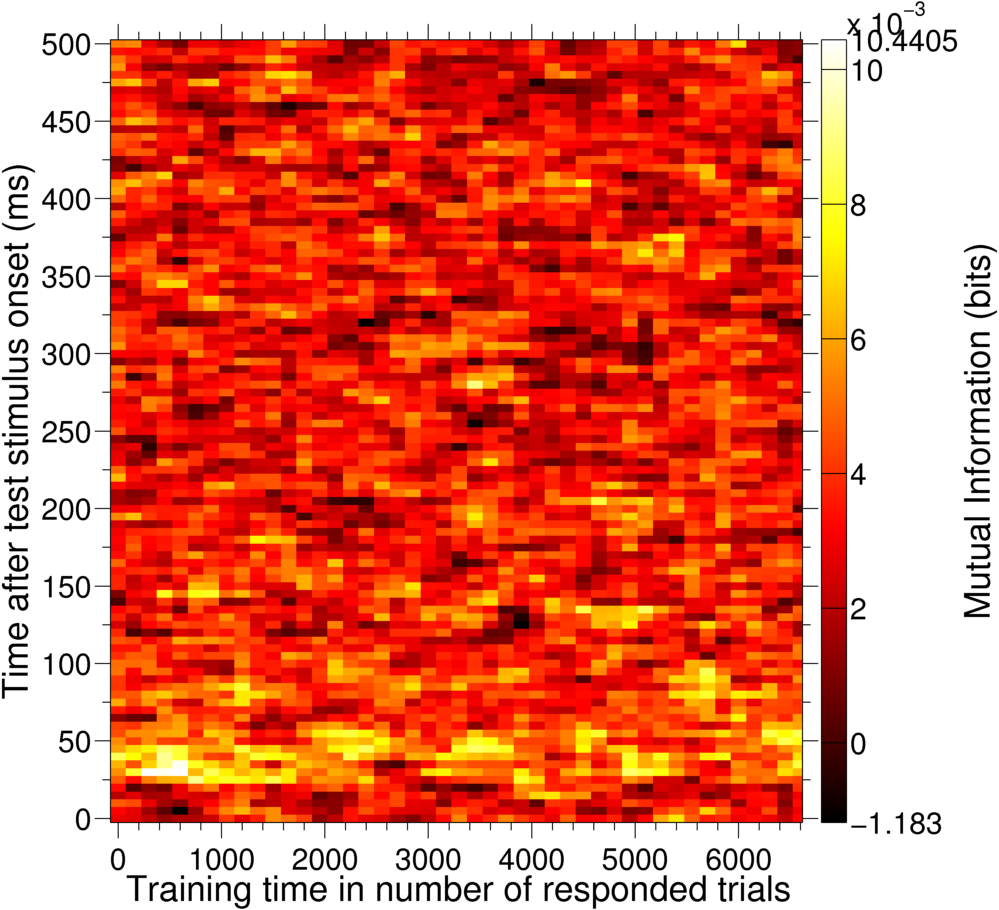
\includegraphics[scale=.25]{%
% % figs/info/I_trialwise_blanco_v1_chmean23_s343-354,355.1,355.2,356-359_tp4_1bins_of_20ms_dr_pt_oc0_test_tc22-3-28,32,35,40_nt600_ts150_rmvet1_rmvms1_pcolorhot_20120816T011920.png}
% %     \end{subfigure}
% %     ~~
% %     \begin{subfigure}[b]{0.5\linewidth}
% %         \centering
% %         \caption{}
% %         \label{fig:j1-1x20fc}
% %         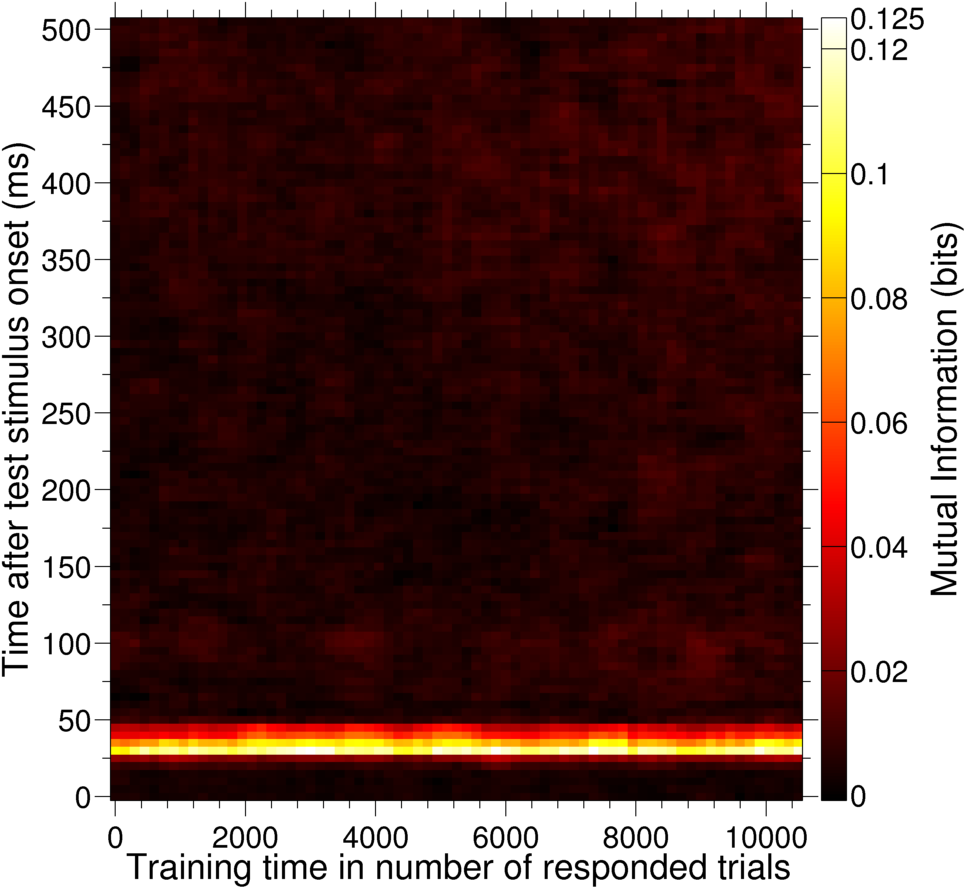
\includegraphics[scale=.25]{%
% % figs/info/I_trialwise_jack_v1_chmean25_s51-72_tp4_1bins_of_20ms_dr_pt_oc0_test_tc22-3-28,32,35,40_nt600_ts150_rmvet1_rmvms1_pcolorhot_20120816T011800.png}
% %     \end{subfigure}
% %     \caption{\ac{V1}: Fine vs. coarse contrast differences.
% % % Mutual information between the test stimulus and \SI{20}{ms} of spiking activity.
% % % The \ac{PT} bias correction method was used in all estimates of the information.
% % In the top panels, the six contrasts included are \{5, 15, 22, 40, 50, 90\}\%; bottom panels \{22, 25, 28, 32, 35, 40\}\%.
% % An average of 100 trials per stimulus is used in each of these.
% % Left panels are for \ac{M1}, right are \ac{M2}.
% % In each case, mutual information between the six test stimuli and \SI{20}{ms} of spiking activity was measured using a spike count code, and bias corrected using the \ac{PT} method.
% % % Panels \ref{fig:b1-1x20cc} and \ref{fig:b1-1x20fc} are for \ac{M1}, \ref{fig:b1-1x20cc} and \ref{fig:b1-1x20fc} for \ac{M2}.
% % }
% %     \label{fig:v1-fvc}
% % \end{figure}


% figs/info/I_trialwise_blanco_v4_chmean31_s307,308,311,313,314,317,318,320,321,329-341_tp4_1bins_of_20ms_dr_pt_oc0_test_tc10-5-20,40-10-60_nt600_ts150_rmvet1_rmvms1_pcolorhot_20120816T012120.png
% figs/info/I_trialwise_blanco_v4_chmean31_s307,308,311,313,314,317,318,320,321,329-341_tp4_1bins_of_20ms_dr_pt_oc0_test_tc27-29,31-33_nt600_ts150_rmvet1_rmvms1_pcolorhot_20120816T011952.png
% figs/info/I_trialwise_jack_v4_chmean20_s24-49_tp4_1bins_of_20ms_dr_pt_oc0_test_tc10-5-20,40-10-60_nt600_ts150_rmvet1_rmvms1_pcolorhot_20120816T011902.png
% figs/info/I_trialwise_jack_v4_chmean20_s24-49_tp4_1bins_of_20ms_dr_pt_oc0_test_tc27-29,31-33_nt600_ts150_rmvet1_rmvms1_pcolorhot_20120816T011843.png

% % \begin{figure}[htbp]
% %     \begin{subfigure}[b]{0.5\linewidth}
% %         \centering
% %         \caption{}
% %         \label{fig:b4-1x20cc}
% %         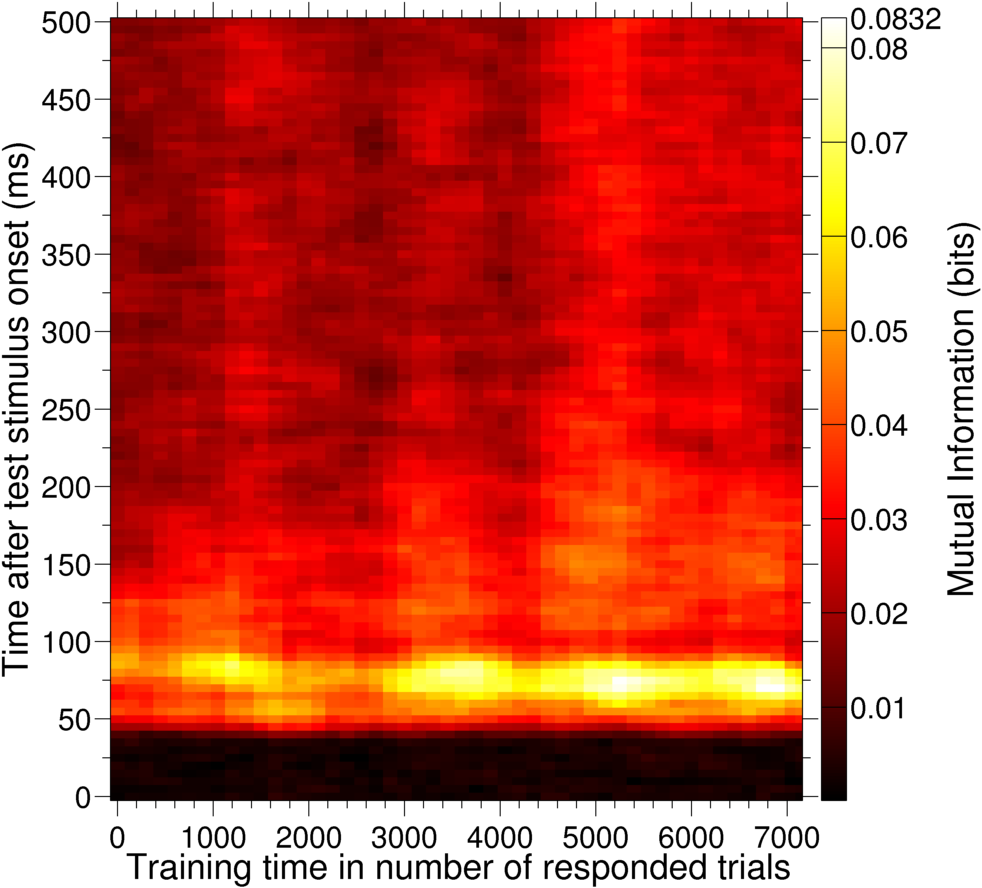
\includegraphics[scale=.25]{%
% % figs/info/I_trialwise_blanco_v4_chmean31_s307,308,311,313,314,317,318,320,321,329-341_tp4_1bins_of_20ms_dr_pt_oc0_test_tc10-5-20,40-10-60_nt600_ts150_rmvet1_rmvms1_pcolorhot_20120816T012120.png}
% %     \end{subfigure}
% %     ~~
% %     \begin{subfigure}[b]{0.5\linewidth}
% %         \centering
% %         \caption{}
% %         \label{fig:j4-1x20cc}
% %         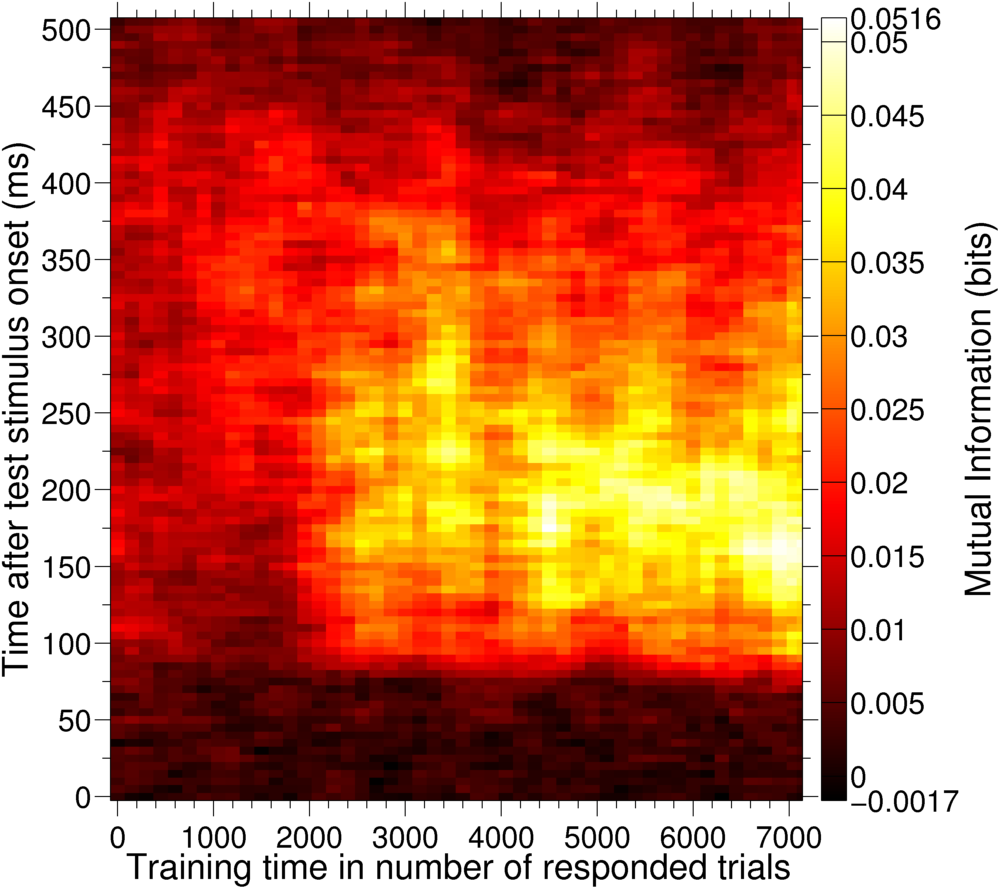
\includegraphics[scale=.25]{%
% % figs/info/I_trialwise_jack_v4_chmean20_s24-49_tp4_1bins_of_20ms_dr_pt_oc0_test_tc10-5-20,40-10-60_nt600_ts150_rmvet1_rmvms1_pcolorhot_20120816T011902.png}
% %     \end{subfigure}
% %     \\
% %     \begin{subfigure}[b]{0.5\linewidth}
% %         \centering
% %         \caption{}
% %         \label{fig:b4-1x20fc}
% %         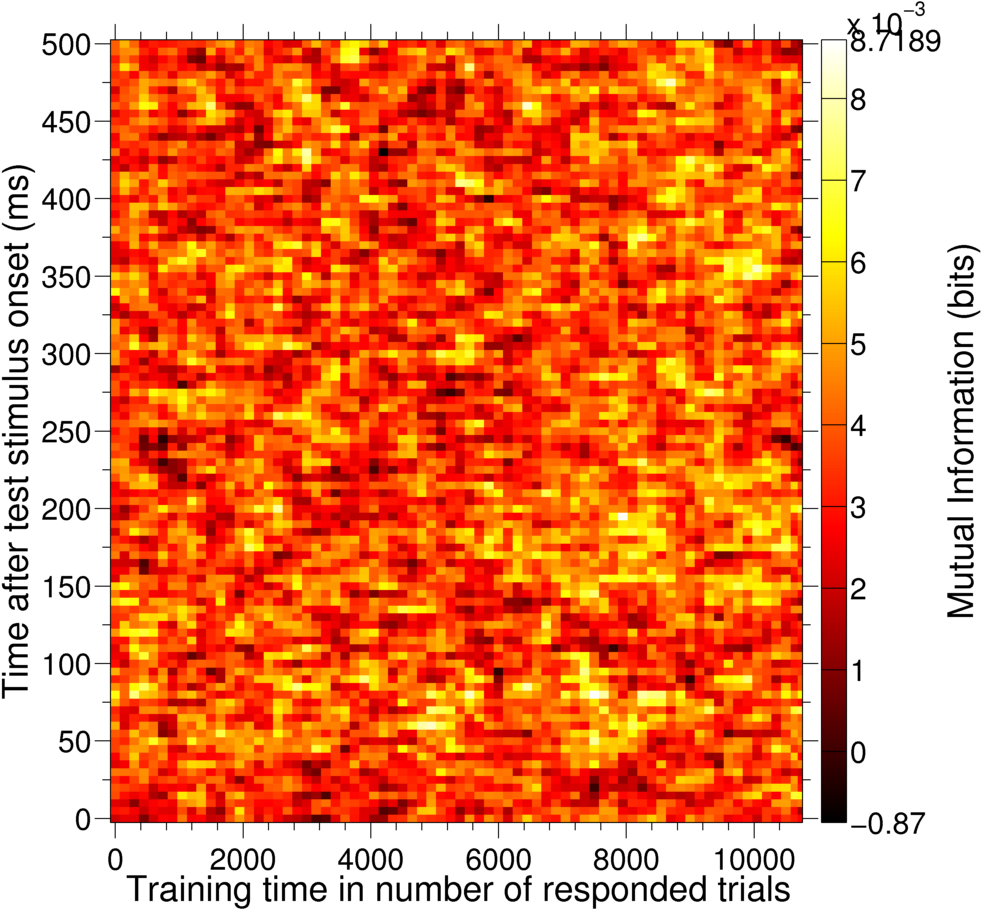
\includegraphics[scale=.25]{%
% % figs/info/I_trialwise_blanco_v4_chmean31_s307,308,311,313,314,317,318,320,321,329-341_tp4_1bins_of_20ms_dr_pt_oc0_test_tc27-29,31-33_nt600_ts150_rmvet1_rmvms1_pcolorhot_20120816T011952.png}
% %     \end{subfigure}
% %     ~~
% %     \begin{subfigure}[b]{0.5\linewidth}
% %         \centering
% %         \caption{}
% %         \label{fig:j4-1x20fc}
% %         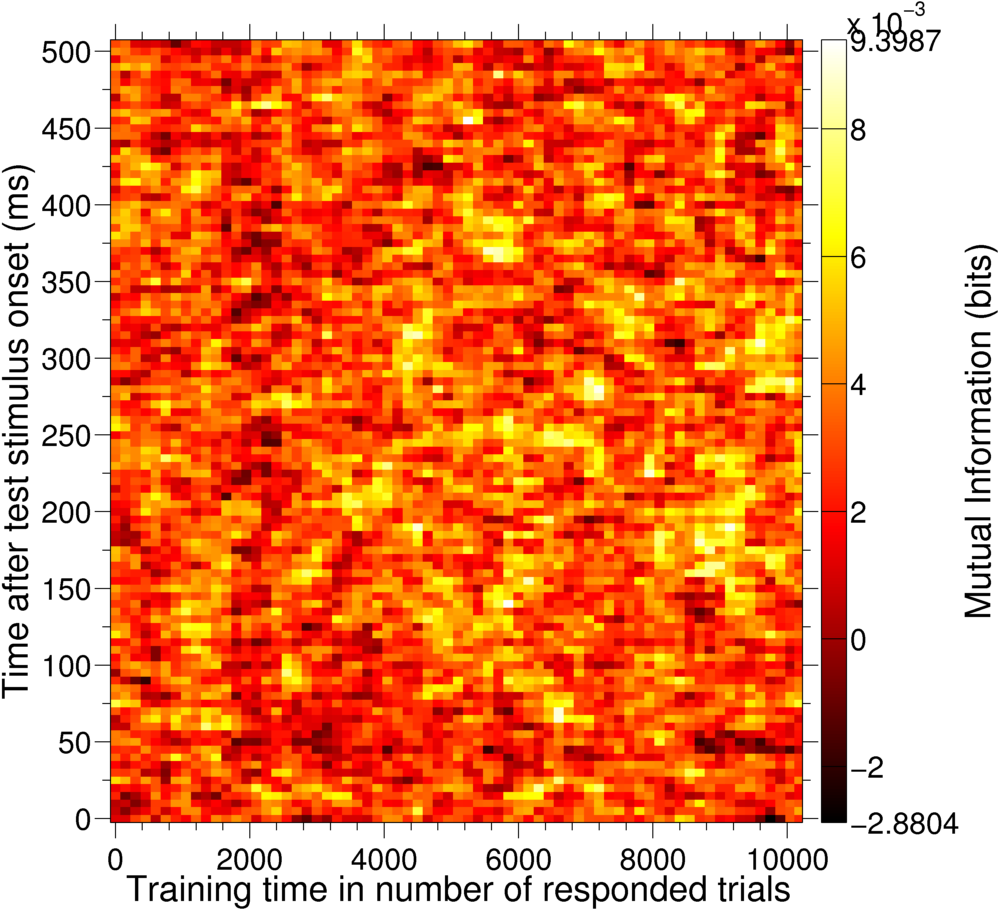
\includegraphics[scale=.25]{%
% % figs/info/I_trialwise_jack_v4_chmean20_s24-49_tp4_1bins_of_20ms_dr_pt_oc0_test_tc27-29,31-33_nt600_ts150_rmvet1_rmvms1_pcolorhot_20120816T011843.png}
% %     \end{subfigure}
% %     \caption{\ac{V4}: Fine vs coarse contrast differences.
% % % Mutual information between the test stimulus and \SI{20}{ms} of spiking activity.
% % % The \ac{PT} bias correction method was used in all estimates of the information.
% % In the top panels, the six contrasts included are \{10, 15, 20, 40, 50, 60\}\%; bottom panels \{27, 28, 29, 31, 32, 33\}\%. An average of 100 trials per stimulus is used in each of these.
% % Left panels are for \ac{M1}, right are \ac{M2}.
% % In each case, mutual information between the six test stimuli and \SI{20}{ms} of spiking activity was measured using a spike count code, and bias corrected using the \ac{PT} method.
% % % Panels \ref{fig:b1-1x20cc} and \ref{fig:b1-1x20fc} are for \ac{M1}, \ref{fig:b1-1x20cc} and \ref{fig:b1-1x20fc} for \ac{M2}.
% % }
% %     \label{fig:v4-fvc}
% % \end{figure}

For \ac{V4}, we find there is no information about fine contrast differences in either animal (Figs.~\ref{fig:b4-1x20fc} and \ref{fig:j4-1x20fc}).
The information about the coarse differences is higher than when all conditions are considered, for reasons discussed above, and these show the same trends as when we analysed all the conditions, in Figs.~\ref{fig:b4-1x20tp4} and \ref{fig:j4-1x20tp4}.

%------------------------------------------------------------------------------
\FloatBarrier
\subsection{Information in millisecond-level spike timing}

For \ac{M2} \ac{V1}, there seems to be some information in the millisecond-level timing of the spikes during the transient response, but not afterward this has elapsed (Fig.~\ref{fig:v1-dif}, right-hand panels).
This band due to the transient is clearly well above the variance of the sampling for the rest of the window offsets.
However, the information in the transient is only present for the coarse contrasts and not for the fine contrasts.
For the fine contrast discrimination in \ac{M2} \ac{V1}, shown in Fig.~\ref{fig:j1-fdif}, (and possibly to a lesser degree on a couple of the other figures) there is an unusual effect where there seems to be more information in the shuffled bins than the unshuffled bins.\footnote{When this is analysed for the raw data with the artifact included, this is subtly more prominently on several of the plots.}

For \ac{M1} \ac{V1}, and also \ac{M1} \ac{V4}, there seems to be an increase in the information contained in the spike timing during the transient also.
However, these results are not as clear-cut as in \ac{M2} \ac{V1}.

% figs/info/I_diff_trialwise_dur=20ms_nshuf=1_blanco_v1_chmean23_s343-354,355.1,355.2,356-359_tp4_dr_pt_oc0_test_tc5-5-20,22-3-28,32,35-5-50,60,90_nt1400_ts350_rmvet1_rmvms1_pcolorbp_20120816T010538.png
% figs/info/I_diff_trialwise_dur=20ms_nshuf=1_blanco_v1_chmean23_s343-354,355.1,355.2,356-359_tp4_dr_pt_oc0_test_tc5,15,22,40,50,90_nt600_ts150_rmvet1_rmvms1_pcolorbp_20120816T004933.png
% figs/info/I_diff_trialwise_dur=20ms_nshuf=1_blanco_v1_chmean23_s343-354,355.1,355.2,356-359_tp4_dr_pt_oc0_test_tc22-3-28,32,35,40_nt600_ts150_rmvet1_rmvms1_pcolorbp_20120816T004908.png
% 
% figs/info/I_diff_trialwise_dur=20ms_nshuf=1_jack_v1_chmean25_s51-72_tp4_dr_pt_oc0_test_tc5-5-20,22-3-28,32,35-5-50,60,90_nt1400_ts350_rmvet1_rmvms1_pcolorbp_20120816T004517.png
% figs/info/I_diff_trialwise_dur=20ms_nshuf=1_jack_v1_chmean25_s51-72_tp4_dr_pt_oc0_test_tc5,15,22,40,50,90_nt600_ts150_rmvet1_rmvms1_pcolorbp_20120816T010526.png
% figs/info/I_diff_trialwise_dur=20ms_nshuf=1_jack_v1_chmean25_s51-72_tp4_dr_pt_oc0_test_tc22-3-28,32,35,40_nt600_ts150_rmvet1_rmvms1_pcolorbp_20120816T004555.png

% % \begin{figure}[htbp]
% %     \begin{subfigure}[b]{0.5\linewidth}
% %         \centering
% %         \caption{}
% %         \label{fig:b1-alldif}
% %         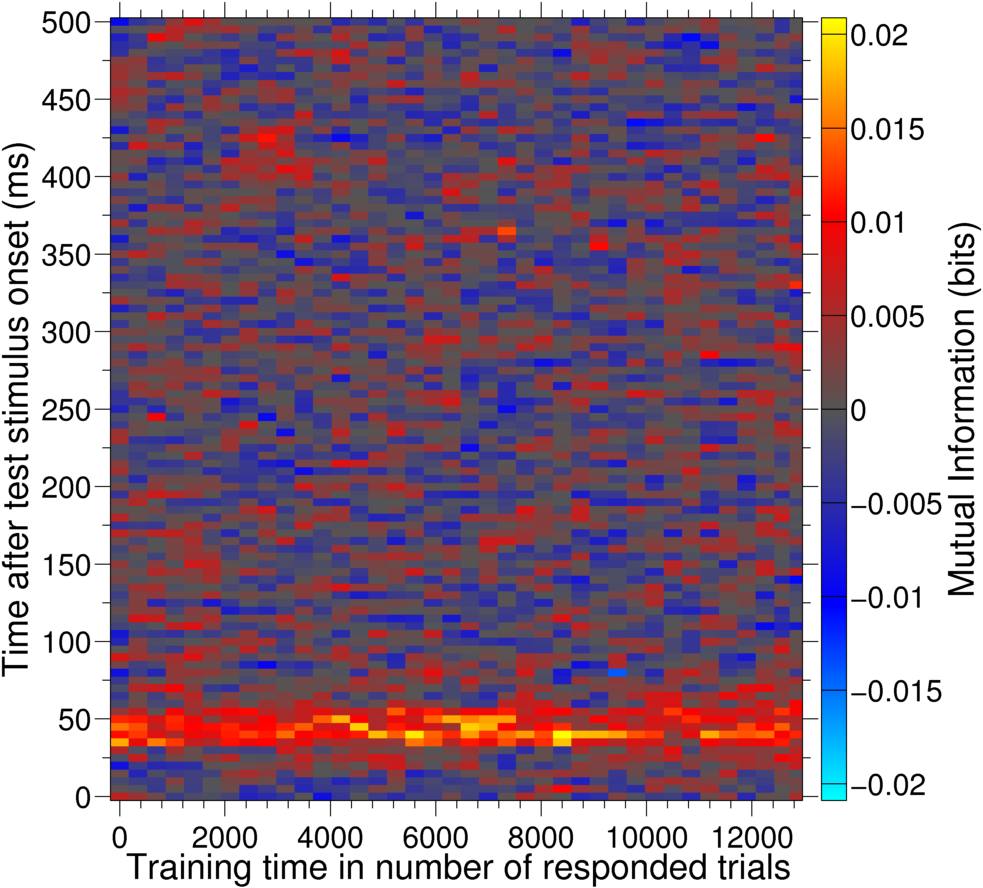
\includegraphics[scale=.25]{%
% % figs/info/I_diff_trialwise_dur=20ms_nshuf=1_blanco_v1_chmean23_s343-354,355.1,355.2,356-359_tp4_dr_pt_oc0_test_tc5-5-20,22-3-28,32,35-5-50,60,90_nt1400_ts350_rmvet1_rmvms1_pcolorbp_20120816T010538.png}
% %     \end{subfigure}
% %     ~~
% %     \begin{subfigure}[b]{0.5\linewidth}
% %         \centering
% %         \caption{}
% %         \label{fig:j1-alldif}
% %         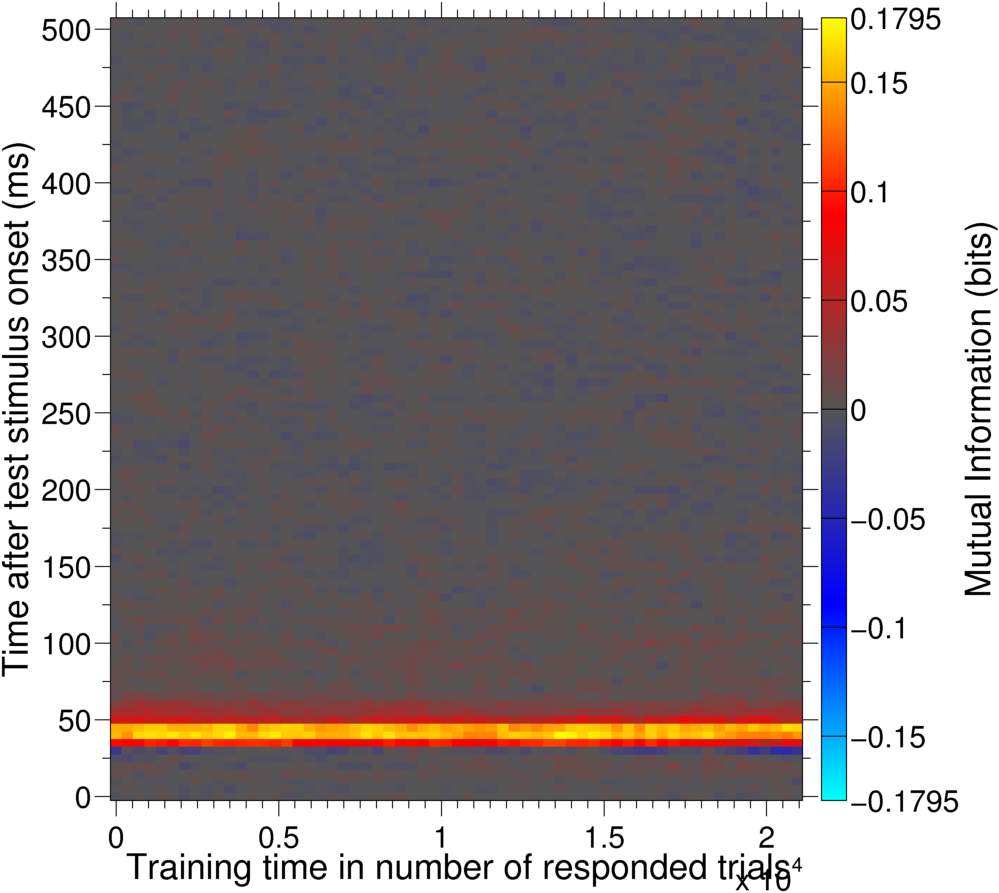
\includegraphics[scale=.25]{%
% % figs/info/I_diff_trialwise_dur=20ms_nshuf=1_jack_v1_chmean25_s51-72_tp4_dr_pt_oc0_test_tc5-5-20,22-3-28,32,35-5-50,60,90_nt1400_ts350_rmvet1_rmvms1_pcolorbp_20120816T004517.png}
% %     \end{subfigure}
% %     \\
% %     \begin{subfigure}[b]{0.5\linewidth}
% %         \centering
% %         \caption{}
% %         \label{fig:b1-cdif}
% %         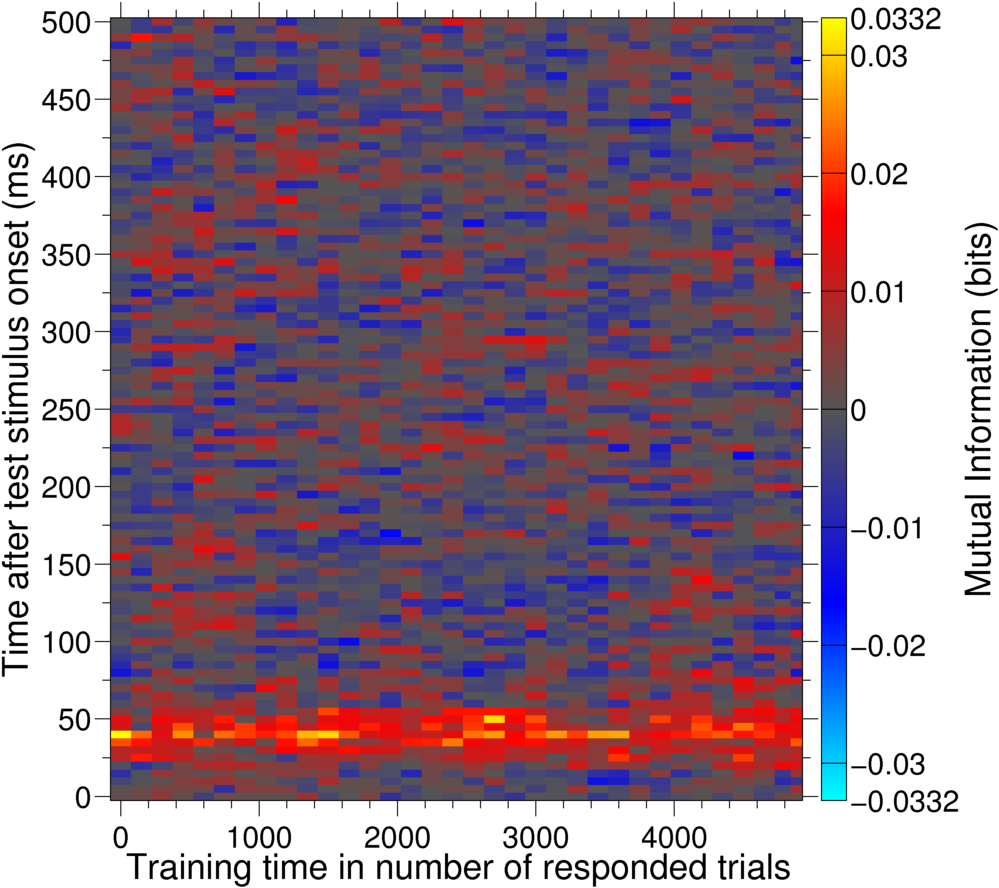
\includegraphics[scale=.25]{%
% % figs/info/I_diff_trialwise_dur=20ms_nshuf=1_blanco_v1_chmean23_s343-354,355.1,355.2,356-359_tp4_dr_pt_oc0_test_tc5,15,22,40,50,90_nt600_ts150_rmvet1_rmvms1_pcolorbp_20120816T004933.png}
% %     \end{subfigure}
% %     ~~
% %     \begin{subfigure}[b]{0.5\linewidth}
% %         \centering
% %         \caption{}
% %         \label{fig:j1-cdif}
% %         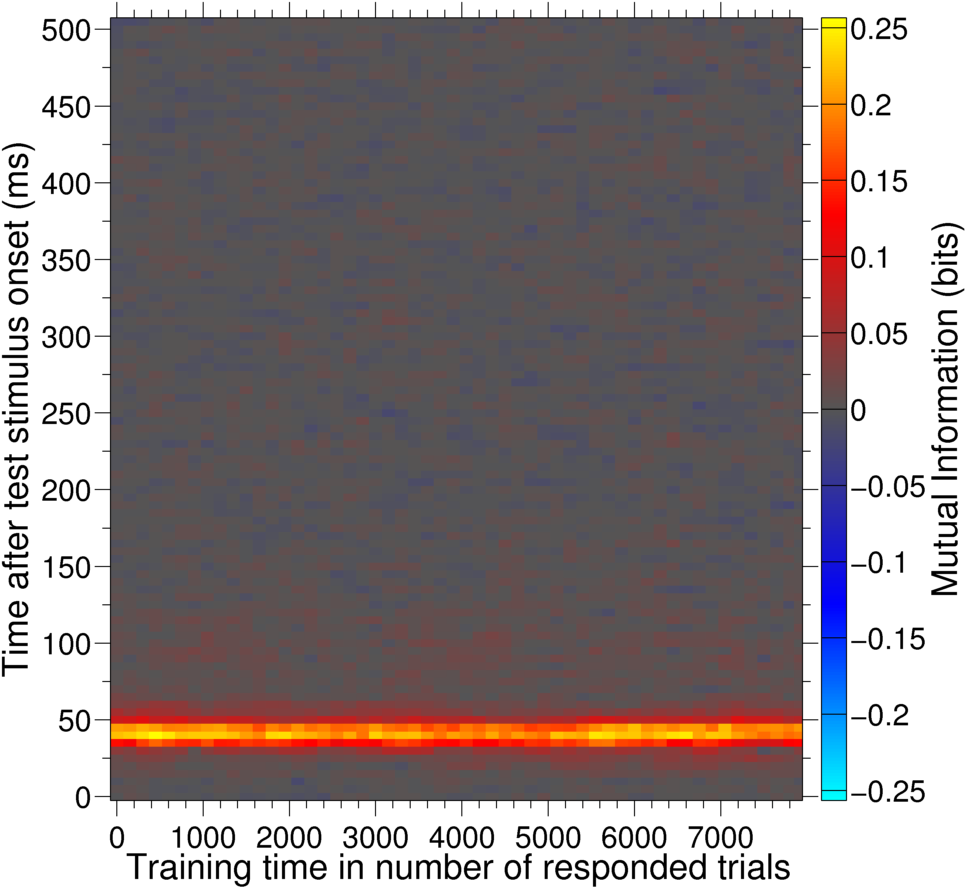
\includegraphics[scale=.25]{%
% % figs/info/I_diff_trialwise_dur=20ms_nshuf=1_jack_v1_chmean25_s51-72_tp4_dr_pt_oc0_test_tc5,15,22,40,50,90_nt600_ts150_rmvet1_rmvms1_pcolorbp_20120816T010526.png}
% %     \end{subfigure}
% %     \\
% %     \begin{subfigure}[b]{0.5\linewidth}
% %         \centering
% %         \caption{}
% %         \label{fig:b1-fdif}
% %         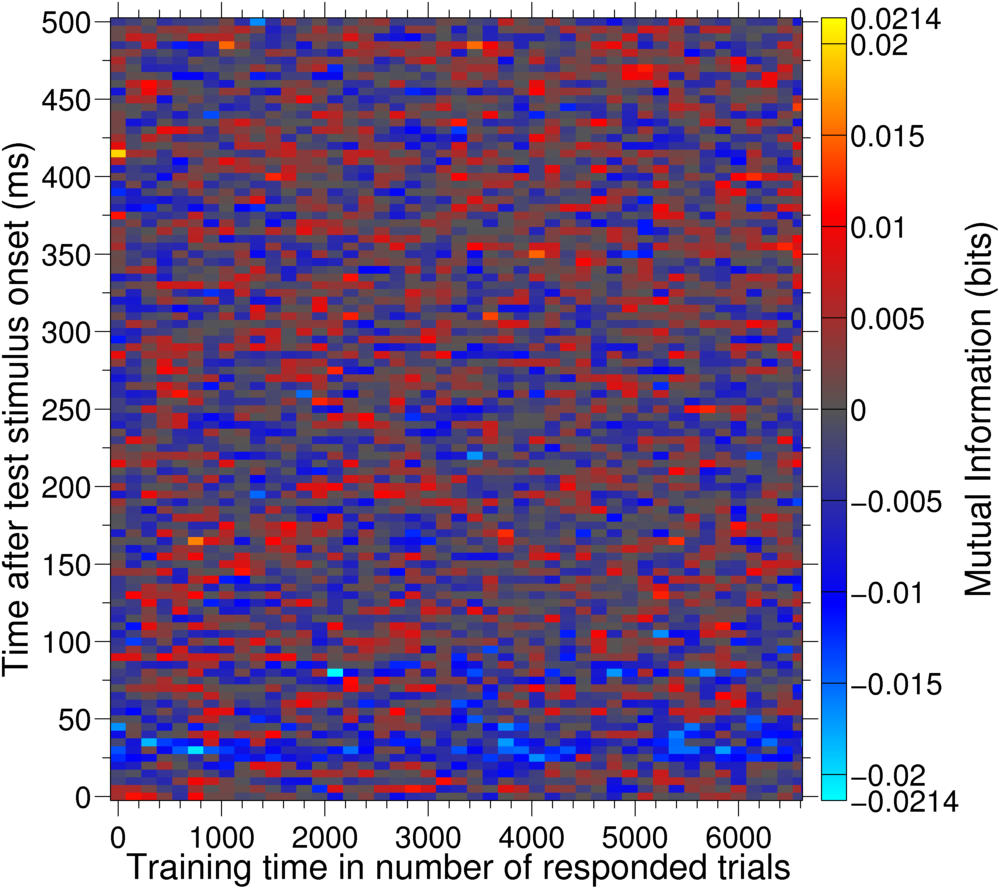
\includegraphics[scale=.25]{%
% % figs/info/I_diff_trialwise_dur=20ms_nshuf=1_blanco_v1_chmean23_s343-354,355.1,355.2,356-359_tp4_dr_pt_oc0_test_tc22-3-28,32,35,40_nt600_ts150_rmvet1_rmvms1_pcolorbp_20120816T004908.png}
% %     \end{subfigure}
% %     ~~
% %     \begin{subfigure}[b]{0.5\linewidth}
% %         \centering
% %         \caption{}
% %         \label{fig:j1-fdif}
% %         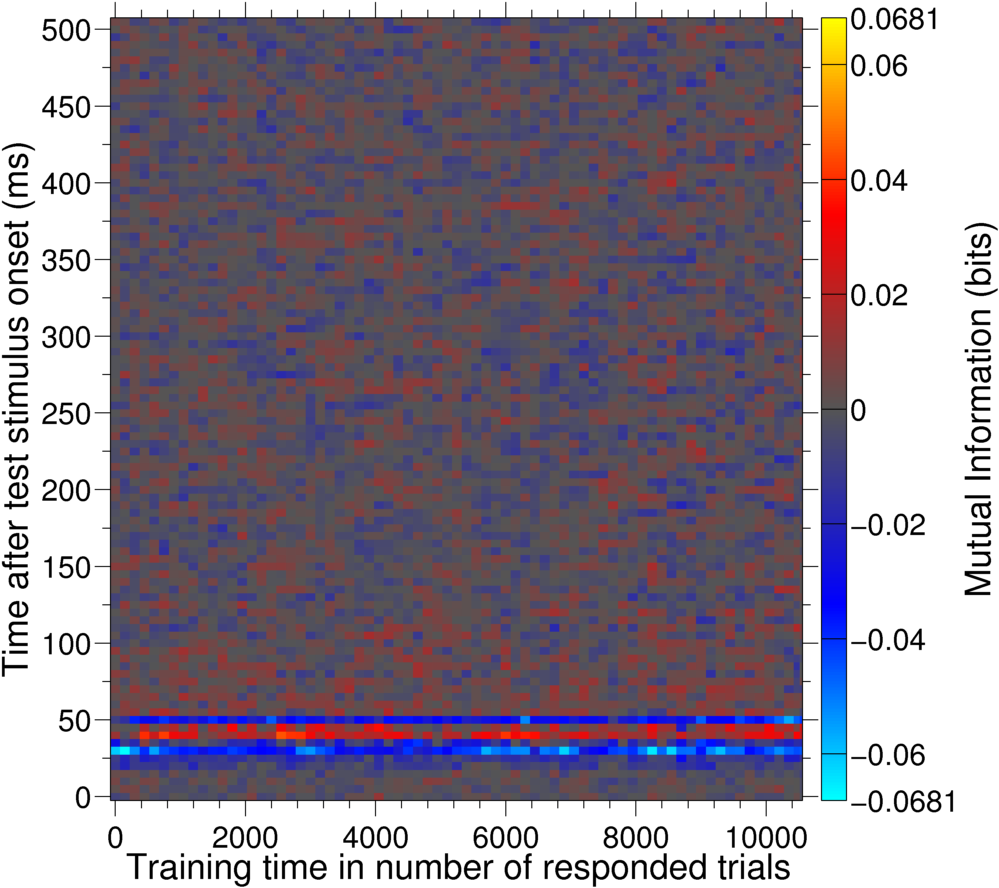
\includegraphics[scale=.25]{%
% % figs/info/I_diff_trialwise_dur=20ms_nshuf=1_jack_v1_chmean25_s51-72_tp4_dr_pt_oc0_test_tc22-3-28,32,35,40_nt600_ts150_rmvet1_rmvms1_pcolorbp_20120816T004555.png}
% %     \end{subfigure}
% %     \caption{\ac{V1}: Information in millisecond level spike timing.
% % % Mutual information between the test stimulus and \SI{20}{ms} of spiking activity.
% % % The \ac{PT} bias correction method was used in all estimates of the information.
% % The information with time-wise shuffled bins was subtracted from information in the spike time code with a \SI{20}{ms} window subdivided into 5 bins.
% % Information was bias corrected using the \ac{PT} method.
% % Left panels: \ac{M1}; Right: \ac{M2}.
% % Top panels: all contrasts, \{10, 15, 20, 25, 27, 28, 29, 31, 32, 33, 35, 40, 50, 60\}\%.
% % Centre panels: \{5, 15, 22, 40, 50, 90\}\%.
% % Bottom panels: \{22, 25, 28, 32, 35, 40\}\%.
% % An average of 100 trials per stimulus is used in the analysis for each.
% % % Panels \ref{fig:b1-1x20cc} and \ref{fig:b1-1x20fc} are for \ac{M1}, \ref{fig:b1-1x20cc} and \ref{fig:b1-1x20fc} for \ac{M2}.
% % }
% %     \label{fig:v1-dif}
% % \end{figure}


% figs/info/I_diff_trialwise_dur=20ms_nshuf=1_blanco_v4_chmean31_s307,308,311,313,314,317,318,320,321,329-341_tp4_dr_pt_oc0_test_tc10-5-20,40-10-60_nt600_ts150_rmvet1_rmvms1_pcolorbp_20120816T011506.png
% figs/info/I_diff_trialwise_dur=20ms_nshuf=1_blanco_v4_chmean31_s307,308,311,313,314,317,318,320,321,329-341_tp4_dr_pt_oc0_test_tc10-5-25,27-29,31-33,35,40-10-60_nt1400_ts350_rmvet1_rmvms1_pcolorbp_20120816T004958.png
% figs/info/I_diff_trialwise_dur=20ms_nshuf=1_blanco_v4_chmean31_s307,308,311,313,314,317,318,320,321,329-341_tp4_dr_pt_oc0_test_tc27-29,31-33_nt600_ts150_rmvet1_rmvms1_pcolorbp_20120816T005048.png
% 
% figs/info/I_diff_trialwise_dur=20ms_nshuf=1_jack_v4_chmean20_s24-49_tp4_dr_pt_oc0_test_tc10-5-20,40-10-60_nt600_ts150_rmvet1_rmvms1_pcolorbp_20120816T213446.png
% figs/info/I_diff_trialwise_dur=20ms_nshuf=1_jack_v4_chmean20_s24-49_tp4_dr_pt_oc0_test_tc10-5-25,27-29,31-33,35,40-10-60_nt1400_ts350_rmvet1_rmvms1_pcolorbp_20120816T004709.png
% figs/info/I_diff_trialwise_dur=20ms_nshuf=1_jack_v4_chmean20_s24-49_tp4_dr_pt_oc0_test_tc27-29,31-33_nt600_ts150_rmvet1_rmvms1_pcolorbp_20120816T004741.png

% % \begin{figure}[htbp]
% %     \begin{subfigure}[b]{0.5\linewidth}
% %         \centering
% %         \caption{}
% %         \label{fig:b4-alldif}
% %         \includegraphics[scale=.25]{%
% % figs/info/I_diff_trialwise_dur=20ms_nshuf=1_blanco_v4_chmean31_s307,308,311,313,314,317,318,320,321,329-341_tp4_dr_pt_oc0_test_tc10-5-25,27-29,31-33,35,40-10-60_nt1400_ts350_rmvet1_rmvms1_pcolorbp_20120816T004958.png}
% %     \end{subfigure}
% %     ~~
% %     \begin{subfigure}[b]{0.5\linewidth}
% %         \centering
% %         \caption{}
% %         \label{fig:j4-alldif}
% %         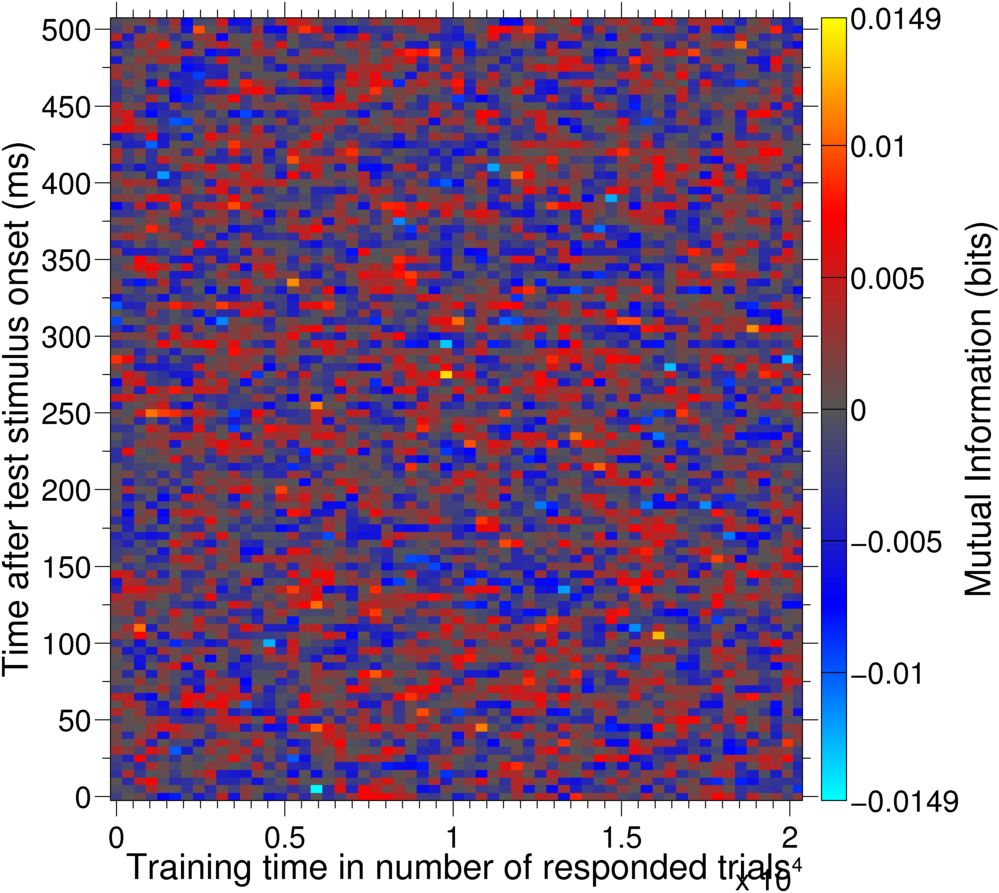
\includegraphics[scale=.25]{%
% % figs/info/I_diff_trialwise_dur=20ms_nshuf=1_jack_v4_chmean20_s24-49_tp4_dr_pt_oc0_test_tc10-5-25,27-29,31-33,35,40-10-60_nt1400_ts350_rmvet1_rmvms1_pcolorbp_20120816T004709.png}
% %     \end{subfigure}
% %     \\
% %     \begin{subfigure}[b]{0.5\linewidth}
% %         \centering
% %         \caption{}
% %         \label{fig:b4-cdif}
% %         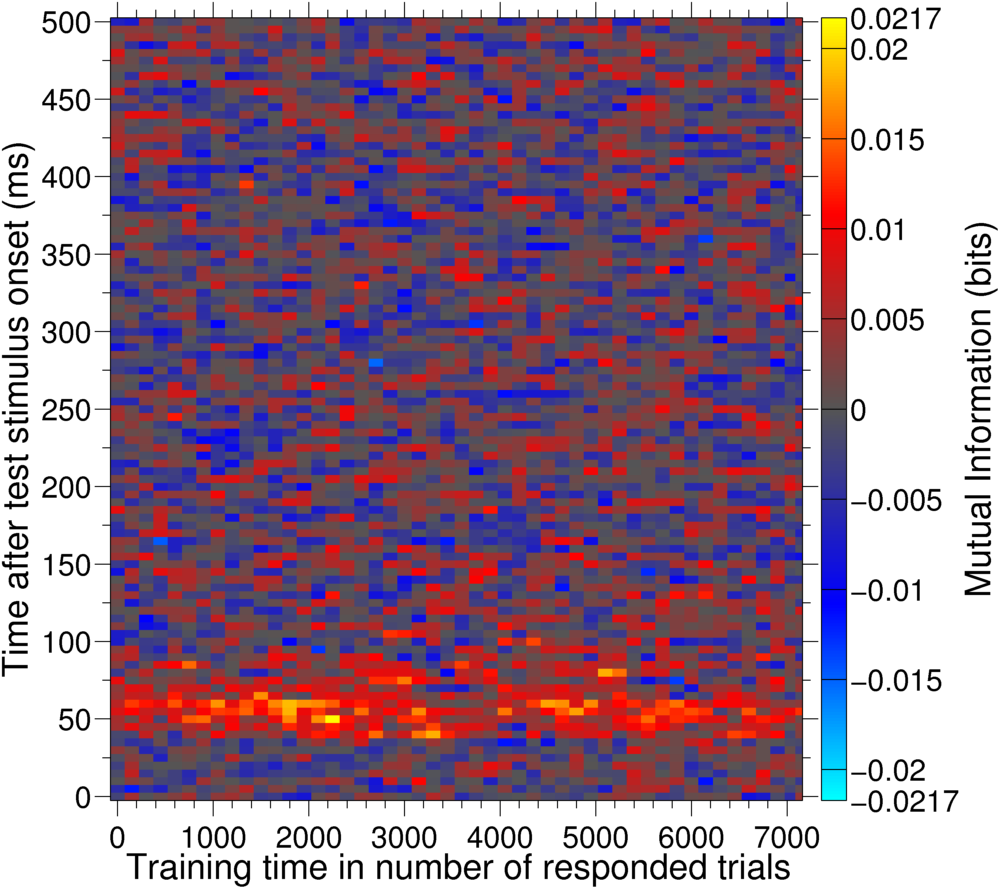
\includegraphics[scale=.25]{%
% % figs/info/I_diff_trialwise_dur=20ms_nshuf=1_blanco_v4_chmean31_s307,308,311,313,314,317,318,320,321,329-341_tp4_dr_pt_oc0_test_tc10-5-20,40-10-60_nt600_ts150_rmvet1_rmvms1_pcolorbp_20120816T011506.png}
% %     \end{subfigure}
% %     ~~
% %     \begin{subfigure}[b]{0.5\linewidth}
% %         \centering
% %         \caption{}
% %         \label{fig:j4-cdif}
% %         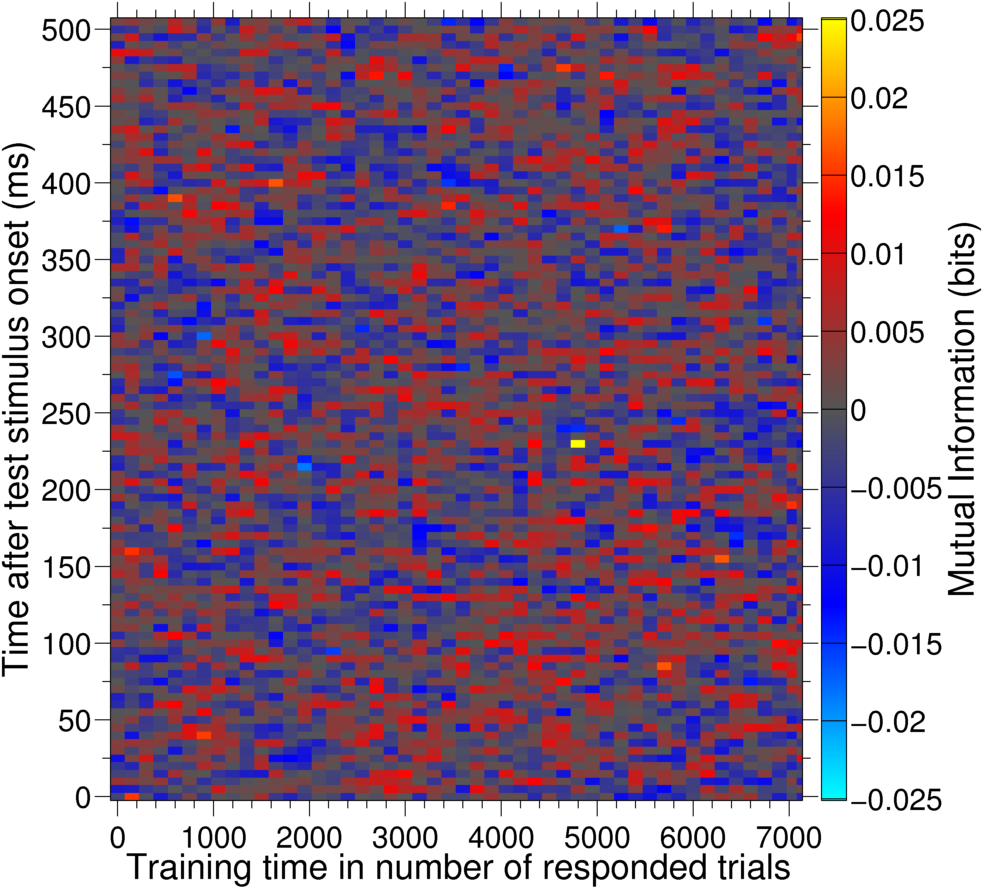
\includegraphics[scale=.25]{%
% % figs/info/I_diff_trialwise_dur=20ms_nshuf=1_jack_v4_chmean20_s24-49_tp4_dr_pt_oc0_test_tc10-5-20,40-10-60_nt600_ts150_rmvet1_rmvms1_pcolorbp_20120816T213446.png}
% %     \end{subfigure}
% %     \\
% %     \begin{subfigure}[b]{0.5\linewidth}
% %         \centering
% %         \caption{}
% %         \label{fig:b4-fdif}
% %         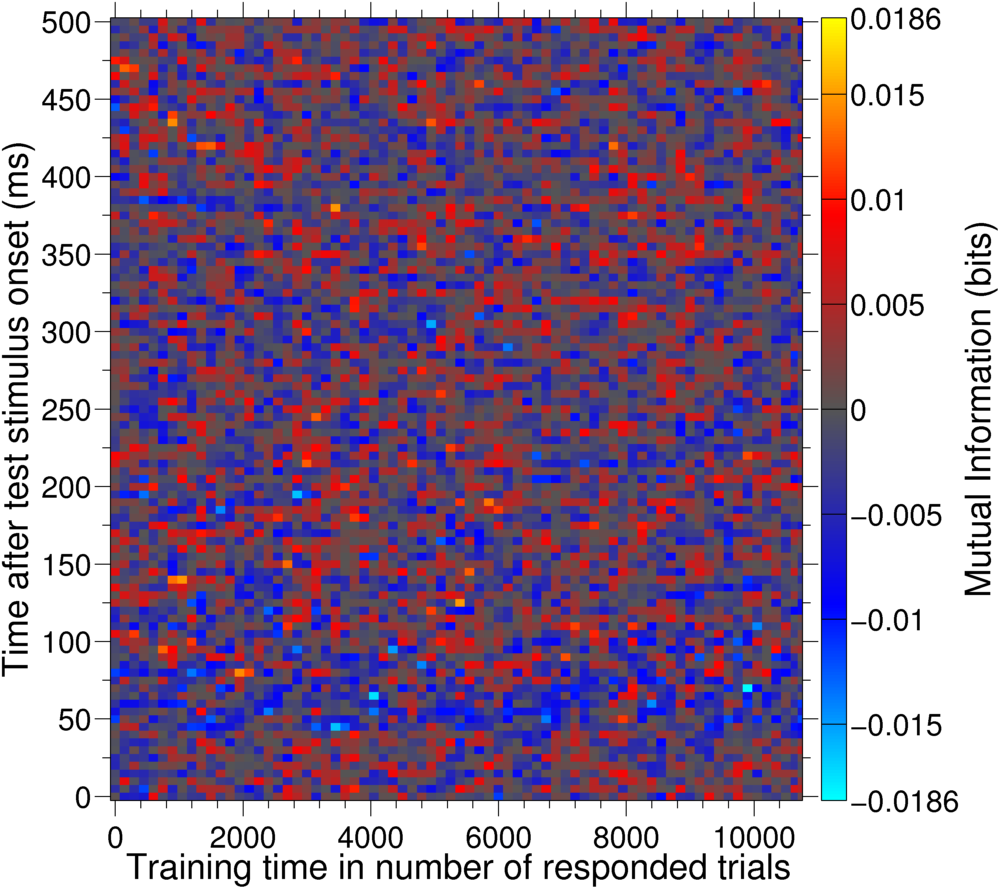
\includegraphics[scale=.25]{%
% % figs/info/I_diff_trialwise_dur=20ms_nshuf=1_blanco_v4_chmean31_s307,308,311,313,314,317,318,320,321,329-341_tp4_dr_pt_oc0_test_tc27-29,31-33_nt600_ts150_rmvet1_rmvms1_pcolorbp_20120816T005048.png}
% %     \end{subfigure}
% %     ~~
% %     \begin{subfigure}[b]{0.5\linewidth}
% %         \centering
% %         \caption{}
% %         \label{fig:j4-fdif}
% %         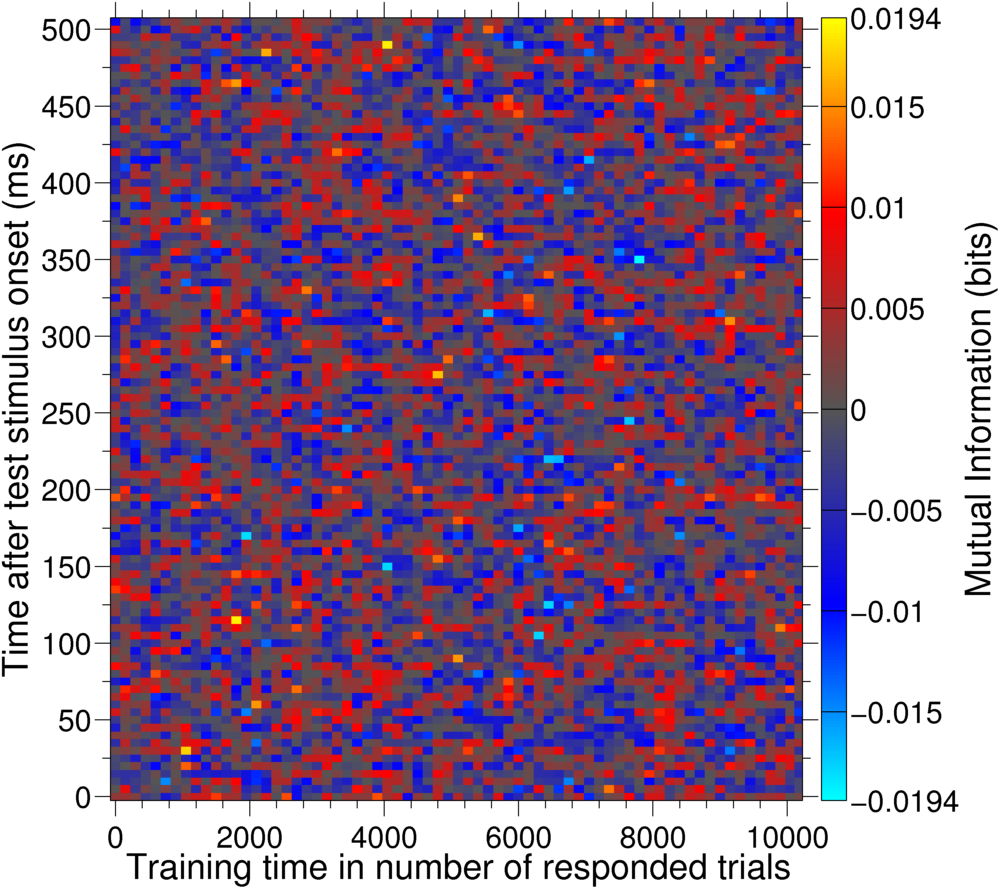
\includegraphics[scale=.25]{%
% % figs/info/I_diff_trialwise_dur=20ms_nshuf=1_jack_v4_chmean20_s24-49_tp4_dr_pt_oc0_test_tc27-29,31-33_nt600_ts150_rmvet1_rmvms1_pcolorbp_20120816T004741.png}
% %     \end{subfigure}
% %     \caption{\ac{V4}: Information in millisecond level spike timing.
% % % Mutual information between the test stimulus and \SI{20}{ms} of spiking activity.
% % % The \ac{PT} bias correction method was used in all estimates of the information.
% % The information with time-wise shuffled bins was subtracted from information in the spike time code with a \SI{20}{ms} window subdivided into 5 bins.
% % Information was bias corrected using the \ac{PT} method.
% % Left panels: \ac{M1}; Right: \ac{M2}.
% % Top panels: all contrasts, \{5, 10, 15, 20, 22, 25, 28, 32, 35, 40, 45, 50, 60, 90\}\%.
% % Centre panels: \{10, 15, 20, 40, 50, 60\}\%.
% % Bottom panels: \{27, 28, 29, 31, 32, 33\}\%.
% % An average of 100 trials per stimulus is used in the analysis for each.
% % % Panels \ref{fig:b1-1x20cc} and \ref{fig:b1-1x20fc} are for \ac{M1}, \ref{fig:b1-1x20cc} and \ref{fig:b1-1x20fc} for \ac{M2}.
% % }
% %     \label{fig:v4-dif}
% % \end{figure}


For \ac{M2} \ac{V4}, there is no information in the spike timing measured on the millisecond timescale: not even during the transient response.

For any of these figures there certainly does not seem to be any change in the information contained in the spike timing alone, so it does not seem to be a trait which can be learned.

% This is true even if we only consider fine contrast differences as well, refuting our hypothesis that there will be more information in the spike timing for more finely differing stimuli contrasts.
% 
% %------------------------------------------------------------------------------
% %------------------------------------------------------------------------------
% %------------------------------------------------------------------------------
% \chapter{$d'$ Analysis}
% %------------------------------------------------------------------------------
% 
% In an attempt to clean up the data and only use the channels and sessions which provide the most relevant results
% 
% Discriminating based on the information content in the channels would allow us to ``cherry-pick'' the best data and artificially inflate the results, so an independent metric of data quality was sought.
% Since we are interested in the channels where the data is of reasonable quality and the neurons represented by the channel are responsive to the stimulus, $d'$ was used.
% 
% $d'$ is ...
% 
% %------------------------------------------------------------------------------
% \subsection{Methods}
% 
% % How is it computed?
% 
% % $$
% % \mu_{stim} = mean(a_{stim});
% % \mu_{spon} = mean(a_{spon});
% % 
% % % Combine the standard deviations of the two sets of trials
% % % Have to do a weighted average of the variances
% % stdev_joint = sqrt(...
% %     ( (n_stim-1)*var(act_stim) + (n_spon-1)*var(act_spon) ) ...
% %     / (n_stim + n_spon - 2) ...
% %     );
% 
% $$
% d\,' = \frac{\mu_{stim} - \mu_{spon}}{\sigma_{joint}}
% ,$$
% where the joint standard deviation over both populations is given by 
% $$
% \sigma_{joint} = \sqrt
%     \frac{ (n_{stim}-1) \, \sigma_{stim} + (n_{spon}-1) \, \sigma_{spon} }
%     { n_{stim} + n_{spon} - 2}
% $$
% so that it is weighted by the number of datapoints, $n_{stim}$ and $n_{spon}$, for both the stimulus presentation and spontaneous activity 
% 
% References
% Compared the mean firing rate for spontaneous activity and the sample stimulus of 30\% contrast
% Compared the mean firing rate for spontaneous activity and the highest contrast test stimulus
% 
% %------------------------------------------------------------------------------
% \subsection{Results}
% 
% d' increases with learning
% 
% Just using channels with a session-wise mean d' > X gives us cleaner results

%------------------------------------------------------------------------------
% \clearpage
\subsection{Decoding}

Fig.~\ref{fig:dec_singles} shows how well the decoder does based only on data from individual channels.
The performance was measured as described in \S\ref{sec:dec-meth-lin} for each session, and then averaged over all sessions.
[perhaps a histogram would show how these are distributed better?]

Fig.~\ref{fig:dec_nbest} indicates how the performance of the decoder improves as more channels are added.
We can see that the decoder performance saturates after around 10 channels are included in the training data, but at a perforance which is still far from the ideal.
After this, including additional channels yields only a slight increase in performance, suggesting nearly all the information contained in the remaining channels is redundant, as it has already been given in the first 10 channels.
[would be better to look at how the decoding perfarmance is distributed across all possible sets of $n$ channels, rather than just the best set of $n$ channels] [this should be compared with shuffled data to see what the impact is and whether performance does not saturate when correlations are removed as per some previous papers [cite]]

NB: the order in which channels were added in Fig.~\ref{fig:dec_nbest} is not the same ordering as they are shown in Fig.~\ref{fig:dec_singles}.

% % \begin{figure}[htbp]
% %     \begin{subfigure}[b]{0.5\linewidth}
% %         \centering
% %         \caption{}
% %         \label{fig:dec_singles}
% %         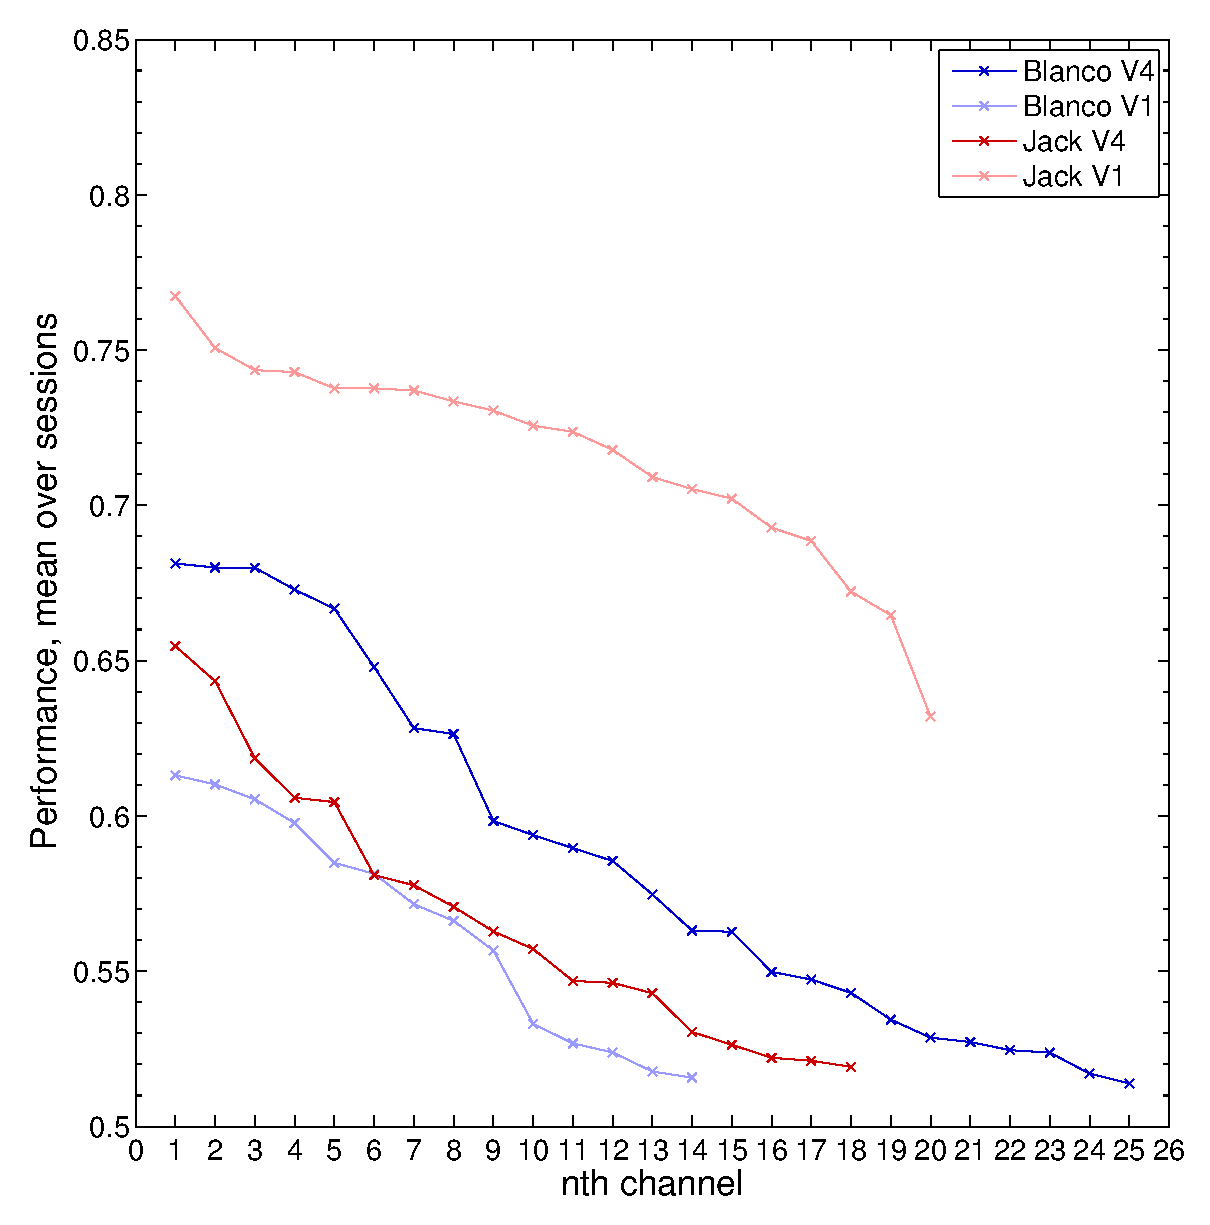
\includegraphics[width=\linewidth]{%
% % figs/decoding/2FC_singles.eps}
% %     \end{subfigure}
% %     ~~
% %     \begin{subfigure}[b]{0.5\linewidth}
% %         \centering
% %         \caption{}
% %         \label{fig:dec_nbest}
% %         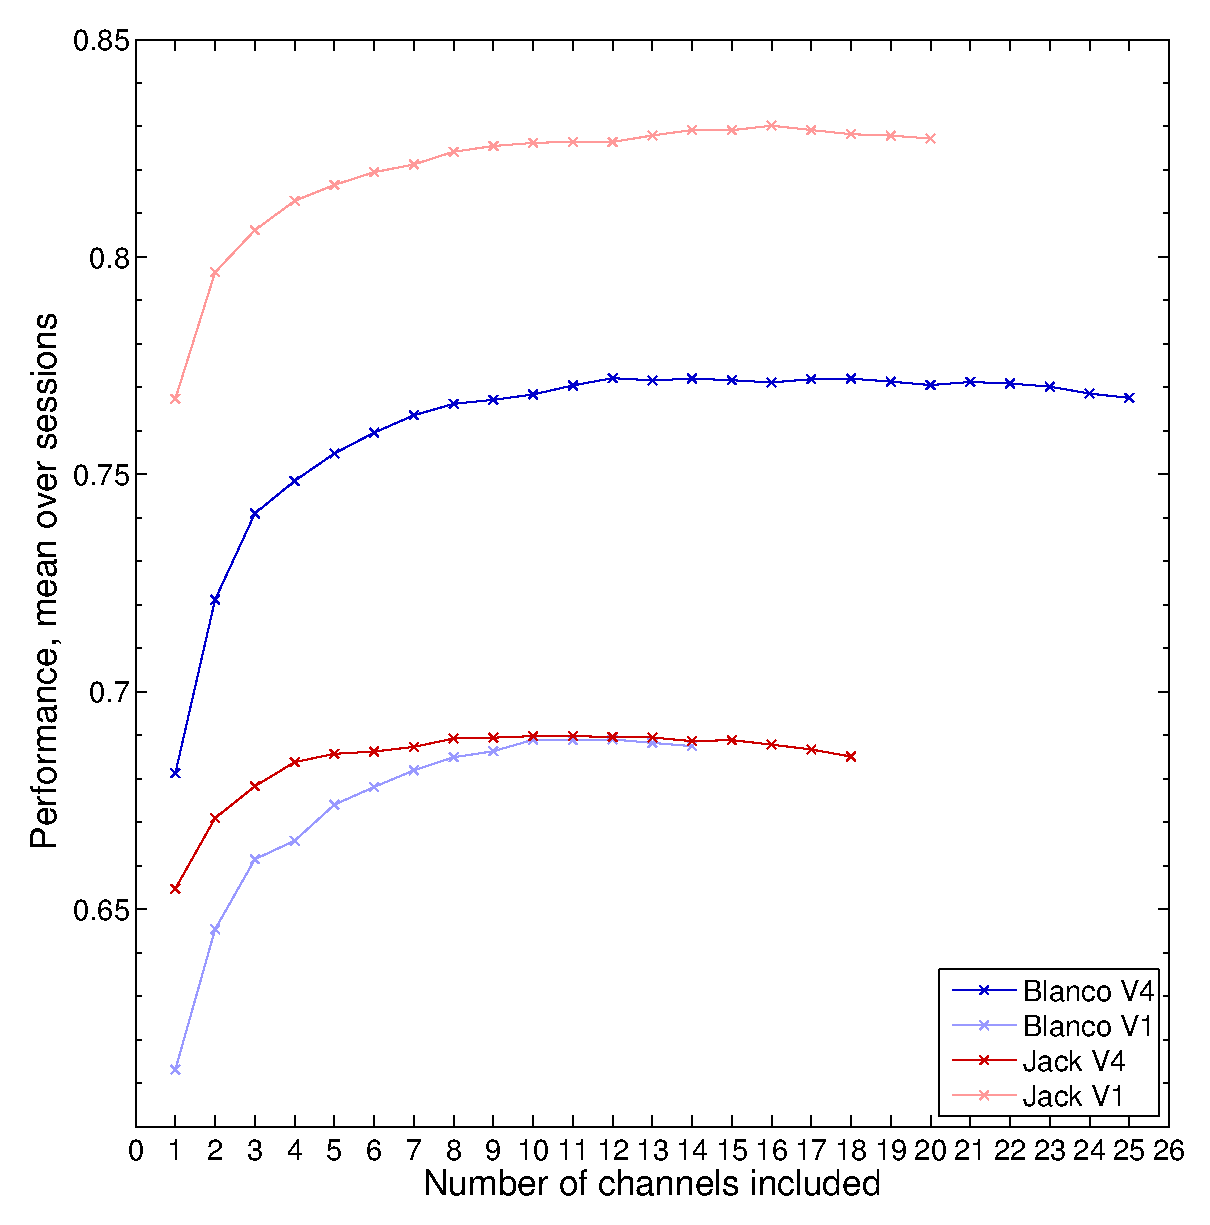
\includegraphics[width=\linewidth]{%
% % figs/decoding/2FC_nbest_all.eps}
% %     \end{subfigure}
% %     \caption{
% % \protect\subref{fig:dec_singles}: Distribution of decoder performance based on spike rate for individual channels, sorted by performance.
% % \protect\subref{fig:dec_nbest}: Decoding performance versus number of channels included in spiking data.
% % Channels were added one at a time, chosen so they maximise the decoder performance for that number of channels whilst keeping all the channels which had come before.
% % }
% %     \label{fig:dec_n}
% % \end{figure}

For each of the datasets, the performance decreases as the last 3 channels are added (Fig.~\ref{fig:dec_nbest}).
I speculate that this is because these channels only contain redundant information, and the increase in dimensionality decreases the quality of the classifier selected from the finite training data available.


% % \begin{figure}[htbp]
% %     \begin{subfigure}[b]{0.5\linewidth}
% %         \centering
% %         \caption{}
% %         \label{fig:dec_b4_allp}
% % 	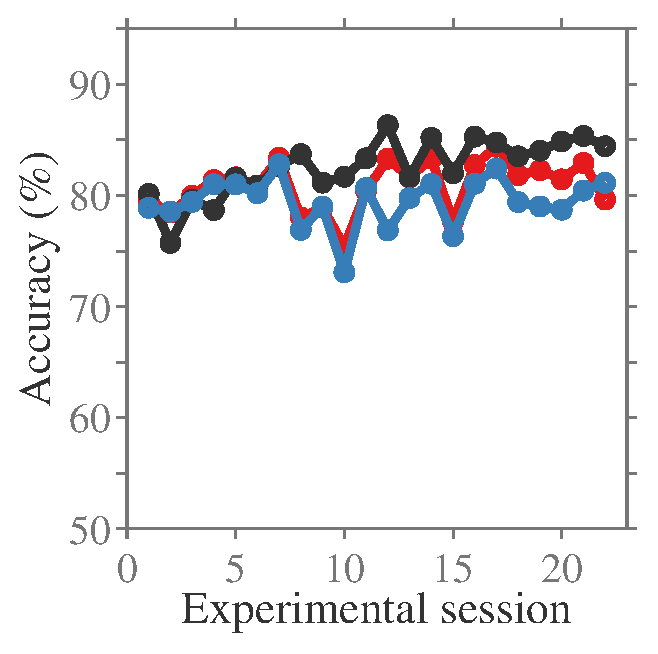
\includegraphics[width=\linewidth]{figs/decoding/perf_v4_blanco.eps}
% %     \end{subfigure}
% %     ~~
% %     \begin{subfigure}[b]{0.5\linewidth}
% %         \centering
% %         \caption{}
% %         \label{fig:dec_j4_allp}
% % 	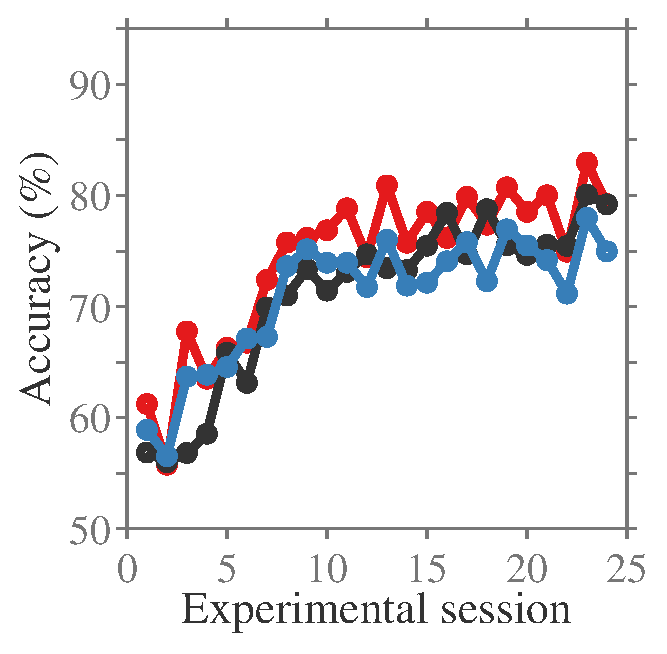
\includegraphics[width=\linewidth]{figs/decoding/perf_v4_jack.eps}
% %     \end{subfigure}
% %     \caption{%
% %     Decoding analysis for \ac{V4}.
% %     Performance of behavioural and decoding predictors by session, averaged across all conditions.
% %     Left panels: \ac{M1}. Right: \ac{M2}.
% % 	Along the x-axis, `Session' is the animal's unique session ID, which increments by one for every day of training.
% %     On the y-axis, `proportion correct' is the proportion of trials for which the response is the same as the target.
% %     This is presented for behavioural performance (black), decoder performance (blue), and decoder performance when trials are shuffled, destroying noise correlations (red; see text).
% % }
% %     \label{fig:dec_all_v4}
% % \end{figure}

% % \begin{figure}[htbp]
% %     \begin{subfigure}[b]{0.5\linewidth}
% %         \centering
% %         \caption{}
% %         \label{fig:dec_b1_allp}
% % 	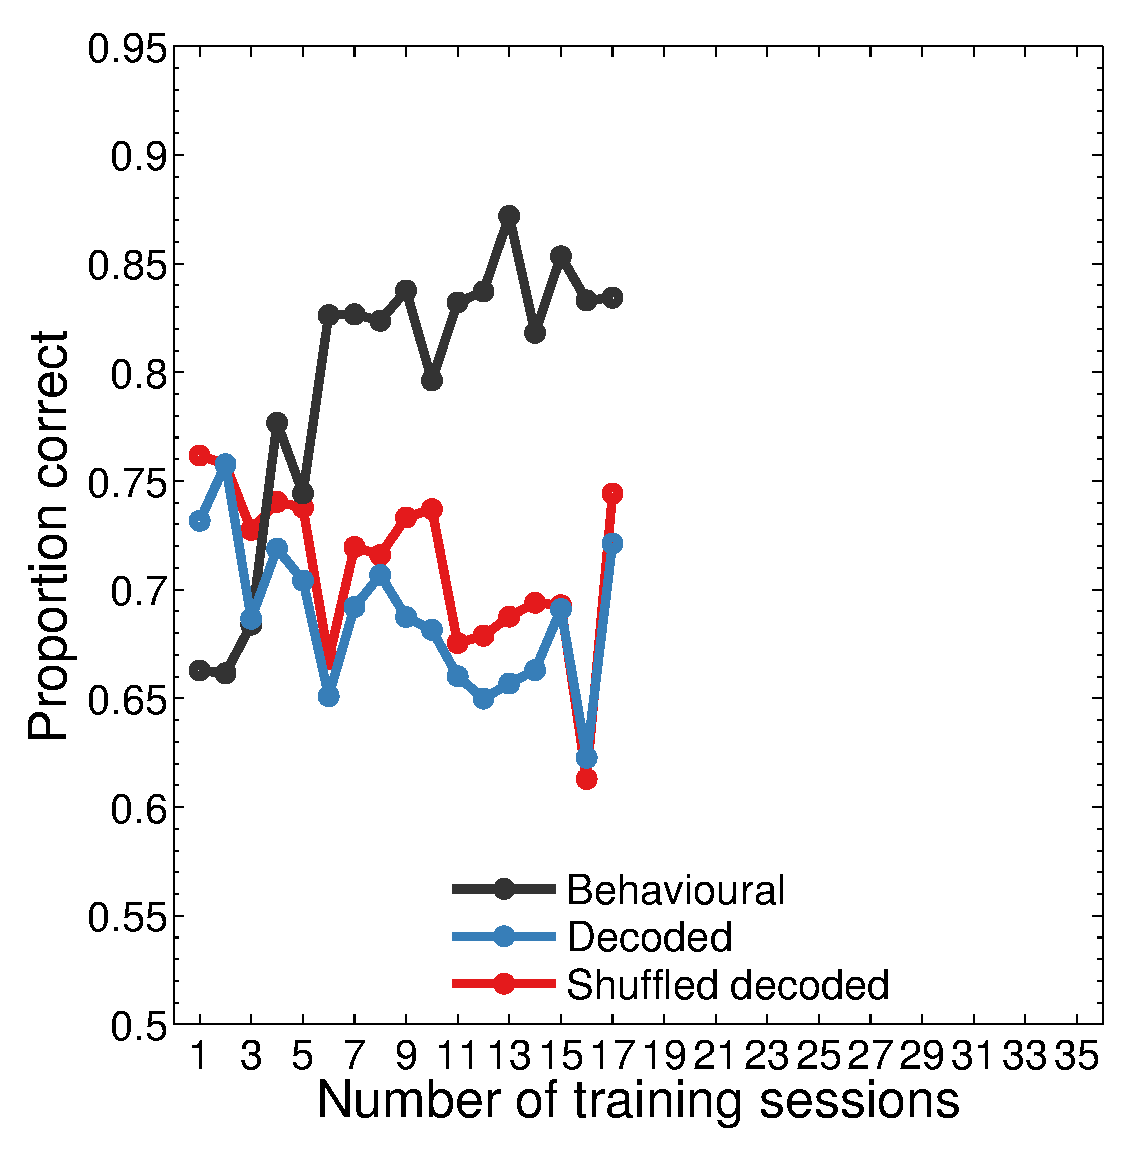
\includegraphics[width=\linewidth]{figs/decoding/perf_v1_blanco.eps}
% %     \end{subfigure}
% %     ~~
% %     \begin{subfigure}[b]{0.5\linewidth}
% %         \centering
% %         \caption{}
% %         \label{fig:dec_j1_allp}
% % 	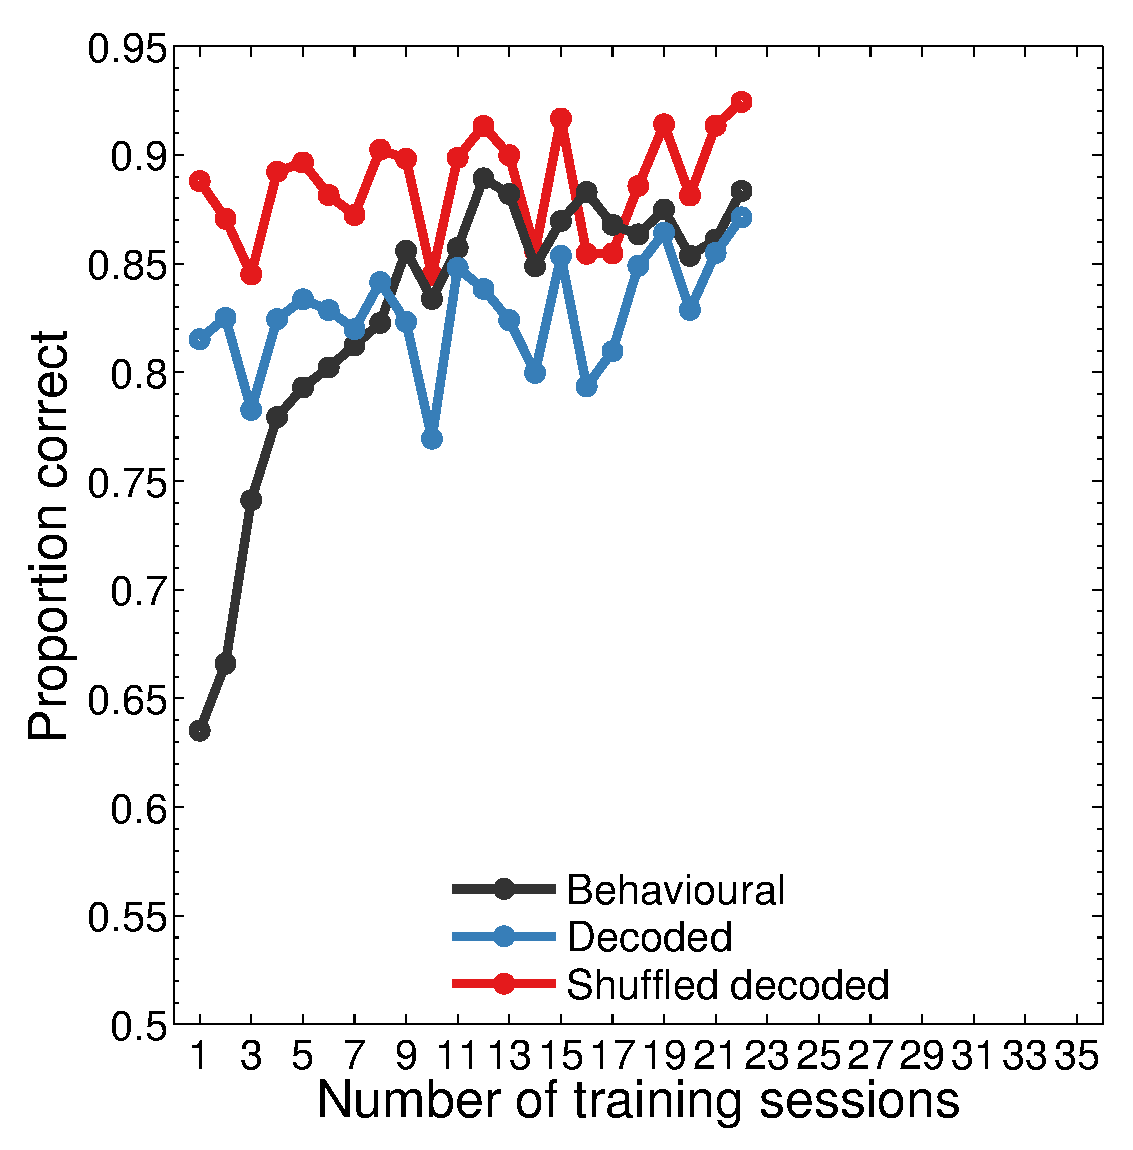
\includegraphics[width=\linewidth]{figs/decoding/perf_v1_jack.eps}
% %     \end{subfigure}
% %     \caption{%
% %     Decoding analysis for \ac{V1}.
% %     Performance of behavioural and decoding predictors by session, averaged across all conditions.
% %     Left panels: \ac{M1}. Right: \ac{M2}.
% % 	Along the x-axis, `Session' is the animal's unique session ID, which increments by one for every day of training.
% %     On the y-axis, `proportion correct' is the proportion of trials for which the response is the same as the target.
% %     This is presented for behavioural performance (black), decoder performance (blue), and decoder performance when trials are shuffled, destroying noise correlations (red; see text).
% % }
% %     \label{fig:dec_all_v1}
% % \end{figure}



For \ac{M2} \ac{V4}, the trend in increase for behavioural performance is well matched by the change in performance of the decoder (Fig.~\ref{fig:dec_j4_allp}, blue and red lines).
In contrast to this, for \ac{M1} \ac{V4} we see the decoding performance is steady despite training, although it should be noted that the increase in behavioural performance was not so large for this animal.

For \ac{M2} \ac{V1}, there is a small gradual increase in decoder performance throughout training, though the increase does not match the timescales and rate of the increase in behavioural performance which is a much sharper transition.
Results for \ac{M2} \ac{V1} could be interpreted as indicating that no further improvements can be obtained from changes in \ac{V1}, and the behavioural performance is limited by the performance of the decoder.
For \ac{M1} \ac{V1}, there is a decrease in decoder in performance despite the increase in behavioural performance (Fig.~\ref{fig:dec_b1_allp}, blue and red lines respectively).


Shuffling the trials to destroy any noise correlations provides an improvement in performance for the data from \ac{M2}, indicating that noise correlations are detrimental to the successful decoding of stimuli.
However, there is no significant difference in decoder performance before and after shuffling for \ac{M1} datasets, which suggests noise correlations have no impact on decoding the contrast of stimuli using firing rate data from a population of neurons.
For \ac{M2} \ac{V1}, the benefit from shuffling seems to be reduced with training; the shuffled decoding performance is reasonably steady throughout training whilst the decoder with noise correlations included increases in performance, closing the gap.

% \marginnote{It might well be better to plot, for each area, the performances for both animals on the same plot and the expected vs observed behavioural agreement for both animals on a seperate plot.}


% % \begin{figure}[htbp]
% %     \begin{subfigure}[b]{0.5\linewidth}
% %         \centering
% %         \caption{}
% %         \label{fig:decag_b4_allp}
% % 	\includegraphics[width=\linewidth]{figs/decoding/agree_v4_blanco.eps}
% %     \end{subfigure}
% %     ~~
% %     \begin{subfigure}[b]{0.5\linewidth}
% %         \centering
% %         \caption{}
% %         \label{fig:decag_j4_allp}
% % 	\includegraphics[width=\linewidth]{figs/decoding/agree_v4_jack.eps}
% %     \end{subfigure}
% %     \caption{%
% %     Decoding analysis for \ac{V4}.
% %     Trial-to-trial agreement between behavioural and decoding predictors.
% %     Left panels: \ac{M1}. Right: \ac{M2}.
% % 	Along the x-axis, `Session' is the animal's unique session ID, which increments by one for every day of training.
% %     On the y-axis is the proportion of trials for which the response is the same as the behavioural response.
% %     The agreement between behaviour and decoding (unshuffled only) is presented alongside the null hypothesis of completely independent binomial distributions.
% %     The dashed line indicates the 95\% confidence interval of the null hypothesis.
% % }
% %     \label{fig:decag_all_v4}
% % \end{figure}

% % \begin{figure}[htbp]
% %     \begin{subfigure}[b]{0.5\linewidth}
% %         \centering
% %         \caption{}
% %         \label{fig:decag_b1_allp}
% % 	\includegraphics[width=\linewidth]{figs/decoding/agree_v1_blanco.eps}
% %     \end{subfigure}
% %     ~~
% %     \begin{subfigure}[b]{0.5\linewidth}
% %         \centering
% %         \caption{}
% %         \label{fig:decag_j1_allp}
% % 	\includegraphics[width=\linewidth]{figs/decoding/agree_v1_jack.eps}
% %     \end{subfigure}
% %     \caption{%
% %     Decoding analysis for \ac{V1}.
% %     Trial-to-trial agreement between behavioural and decoding predictors.
% %     Left panels: \ac{M1}. Right: \ac{M2}.
% % 	Along the x-axis, `Session' is the animal's unique session ID, which increments by one for every day of training.
% %     On the y-axis is the proportion of trials for which the response is the same as the behavioural response.
% %     The agreement between behaviour and decoding (unshuffled only) is presented alongside the null hypothesis of completely independent binomial distributions.
% %     The dashed line indicates the 95\% confidence interval of the null hypothesis.
% % }
% %     \label{fig:decag_all_v1}
% % \end{figure}


With regards to the behavioural and decoding response agreement, we find there is no consistent significant deviation from the null hypothesis for \ac{V1} data.
There are a couple of sessions where unshuffled agreement is above the boundary for significance for each of the animals, but this is not a consistent effect.
The agreement between shuffled decoding and behaviour does not deviate from the corresponding null hypothesis.
This shows that the shuffled is higher than the unshuffled decoding agreement only because the shuffled decoder is more accurate at matching the target response.

For \ac{V4}, we see that the agreement does not deviate significantly from the null hypothesis for earlier sessions, but after a cut off point all later sessions do (\ac{M1}: all sessions before 321 are not, after 329 are significant; \ac{M2}: Before 28 are not, after 28 are significant).
The effect is stronger for \ac{M2}, but present for both animals.
This indicates that the behavioural responses and the decoded responses based on the neural data were not notably correlated, but have become so with training.

Because the shuffled decoded responses are more accurate (with respect to the target response), they are predicted under the null hypothesis to be in better agreement with the behavioural responses.
However we observe these are in worse agreement than the unshuffled decoding, and do not deviate from the corresponding NH line.

A more detailed breakdown of these results with subsets of the 14 conditions is given in Figs.~\ref{fig:dec_detail_b1} and \ref{fig:dec_detail_j4}.
Comparing Figs.~\ref{fig:dec_b4_6easy_a} and \ref{fig:dec_j4_6easy_a} with Figs.~\ref{fig:dec_b4_6hard_a} and \ref{fig:dec_j4_6hard_a}, we can see that the decoding responses for the easier conditions fit the null hypothesis model, whilst the more challenging conditions do not and have a statistically significant agreement with the animal behaviour.




%------------------------------------------------------------------------------
\clearpage
\subsection{Noise correlations}
%------------------------------------------------------------------------------

For both \ac{V1} and \ac{V4}, the average noise correlation between pairs of channels seem to remain stable for \ac{M1} and decrease by a small margin for \ac{M2} (see Fig.~\ref{fig:noise_r_all}).
The increase in noise correlation for \ac{M1} \ac{V1} for the last two sessions (session numbers 358 and 359) is due to a decline in data quality and an increase in noise from artificial sources.
There is a large amount of variance in the noise correlations for different pairs, so the decline in mean correlation for \ac{M2} does not seem very large considering the amount of variance.


% % \begin{figure}[htb]
% %     \begin{subfigure}[b]{0.5\linewidth}
% %         \centering
% %         \caption{}
% %         \label{fig:noise_r_v1_all}
% % %         \includegraphics[width=\linewidth]{%
% % % ./rcoef_2013-04-09/rcoef_sess_meanpc_2013-04-09/png/rcoef_sess_meanpc_v1_both.png}
% % %        \includegraphics[width=\linewidth]{figs/decoding/rcoef_sess_meanpc_v1_both}
% %         \includegraphics[width=\linewidth]{figs/decoding/rcoef_sess_meanpc_v1_both.pdf}
% %     \end{subfigure}
% %     ~~
% %     \begin{subfigure}[b]{0.5\linewidth}
% %         \centering
% %         \caption{}
% %         \label{fig:noise_r_v4_all}
% % %         \includegraphics[width=\linewidth]{%
% % % ./rcoef_2013-04-09/rcoef_sess_meanpc_2013-04-09/png/rcoef_sess_meanpc_v4_both.png}
% %         \includegraphics[width=\linewidth]{figs/decoding/rcoef_sess_meanpc_v4_both.pdf}
% %     \end{subfigure}
% %     \caption{Change in noise correlations with learning.
% % \protect\subref{fig:noise_r_v1_all}:~\ac{V1}.
% % \protect\subref{fig:noise_r_v4_all}:~\ac{V4}.
% % Blue:~\ac{M1}.
% % Red:~\ac{M2}.
% % On the x-axis, the number of sessions since the animal began training in the part of the visual field retinotopic to the recording site is shown.
% % Line: pearson r coefficient, averaged across the possible pairings between channels for each of the 14 trial conditions.
% % Shaded region indicates one standard deviation from mean.
% % }
% %     \label{fig:noise_r_all}
% % \end{figure}
% \marginnote{In Fig.~\ref{fig:noise_r_all} and \ref{fig:noise_r_hist}, the text is too small due to saving the figure with transparencies in PNG format; if I could get the SVG to load correctly, the text would be sized correctly.}

Fig.~\ref{fig:noise_r_hist} is intended to reproduce Figure 2C from \citet{Gu2011}, with the distribution of $r$ shown across pairs for one pre-training and one post-training session.
These sessions were chosen from a restricted set of sessions which did not have problems with artificially high correlations from the motion artifact, and selected from this set such that they were as close to the start and end of the training period as possible.
However, this selection was made before the set of trials was redacted as mentioned in \S\ref{sec:dec-meth-noise}, so the sessions selected could possibly be made further apart.

The data presented in Fig.~\ref{fig:noise_r_hist} shows that the distribution of noise correlation pairs does not move significantly for \ac{M1} \ac{V1}, which is contrasted by a clear decrease for \ac{M2} \ac{V1}.
It should be noted though that the distribution for \ac{M2} \ac{V1} begins higher than \ac{M1} and decreases to a similar value as \ac{M1} \ac{V1}.
For \ac{V4}, there is an increase in mean noise correlation for \ac{M1} and a decrease for \ac{M2}, though as \ac{M2} begins higher than \ac{M1} the two do tend toward to one another.

Cherry-picking is a significant problem here, as there is sizable day-to-day variation in the noise correlation across the pairs.
Choosing a session where there is more noise correlation than neighbouring sessions at the beginning of training and less at the end of training will give the impression that there is a more significant decrease in noise correlations.
More effort should be made to counter inadvertently cherry-picking in the session selection, as Fig.~\ref{fig:noise_r_j1_pmc} indicates this may be one reason for such a sizable decrease in noise correlation for \ac{M2} \ac{V1}.

% % \begin{figure}[htbp]
% %     \begin{subfigure}[b]{0.5\linewidth}
% %         \centering
% %         \caption{}
% %         \label{fig:noise_r_b1_hist}
% % %         \includegraphics[width=\linewidth]{%
% % % ./rcoef_2013-03-25/rcoef_sess_histallover_2013-03-25/png/rcoef_sess_histallover_v1_blanco.png}
% %         \includegraphics[width=\linewidth]{figs/decoding/rcoef_sess_histallover_v1_blanco.pdf}
% %     \end{subfigure}
% %     ~~
% %     \begin{subfigure}[b]{0.5\linewidth}
% %         \centering
% %         \caption{}
% %         \label{fig:noise_r_j1_hist}
% % %         \includegraphics[width=\linewidth]{%
% % % ./rcoef_2013-03-25/rcoef_sess_histallover_2013-03-25/png/rcoef_sess_histallover_v1_jack.png}
% %         \includegraphics[width=\linewidth]{figs/decoding/rcoef_sess_histallover_v1_jack.pdf}
% %     \end{subfigure}
% %     \\
% %     \begin{subfigure}[b]{0.5\linewidth}
% %         \centering
% %         \caption{}
% %         \label{fig:noise_r_b4_hist}
% % %         \includegraphics[width=\linewidth]{%
% % % ./rcoef_2013-03-25/rcoef_sess_histallover_2013-03-25/png/rcoef_sess_histallover_v4_blanco.png}
% %         \includegraphics[width=\linewidth]{figs/decoding/rcoef_sess_histallover_v4_blanco.pdf}
% %     \end{subfigure}
% %     ~~
% %     \begin{subfigure}[b]{0.5\linewidth}
% %         \centering
% %         \caption{}
% %         \label{fig:noise_r_j4_hist}
% % %         \includegraphics[width=\linewidth]{%
% % % ./rcoef_2013-03-25/rcoef_sess_histallover_2013-03-25/png/rcoef_sess_histallover_v4_jack.png}
% %         \includegraphics[width=\linewidth]{figs/decoding/rcoef_sess_histallover_v4_jack.pdf}
% %     \end{subfigure}
% %     \caption{Distribution of the noise correlations for the pairings across all conditions.
% % Two sessions, one at the beginning of training (black) and one at the end of training (red) are shown for comparitive purposes.
% % \protect\subref{fig:noise_r_b1_hist}: \ac{M1} \ac{V1}; sessions 343 and 354.
% % \protect\subref{fig:noise_r_j1_hist}: \ac{M2} \ac{V1}; sessions 51 and 71.
% % \protect\subref{fig:noise_r_b4_hist}: \ac{M1} \ac{V4}; sessions 307 and 338.
% % \protect\subref{fig:noise_r_j4_hist}: \ac{M2} \ac{V4}; sessions 27 and 46.
% % }
% %     \label{fig:noise_r_hist}
% % \end{figure}


% Fig.~\ref{fig:noise_r_pmc} indicates that noise correlations are correlated for pairs across sessions.
A pairs of channels which have higher noise correlations in one session are likely to have higher noise correlation in other sessions.
However, this effect is not present for \ac{M1} \ac{V1}, Fig.~\ref{fig:noise_r_b1_pmc}, and could suggest there is less session-to-session consistency for this dataset.

This figure provides an easy way of visually inspecting whether noise correlations are conserved, but does not allow us to quantify this.

% % \begin{figure}[htbp]
% %     \begin{subfigure}[b]{0.5\linewidth}
% %         \centering
% %         \caption{}
% %         \label{fig:noise_r_b1_pmc}
% %         \includegraphics[width=\linewidth]{%
% % figs/decoding/rcoef_sess_pairsmeanc_v1_blanco.eps}
% %     \end{subfigure}
% %     ~~
% %     \begin{subfigure}[b]{0.5\linewidth}
% %         \centering
% %         \caption{}
% %         \label{fig:noise_r_j1_pmc}
% %         \includegraphics[width=\linewidth]{%
% % figs/decoding/rcoef_sess_pairsmeanc_v1_jack.eps}
% %     \end{subfigure}
% %     \\
% %     \begin{subfigure}[b]{0.5\linewidth}
% %         \centering
% %         \caption{}
% %         \label{fig:noise_r_b4_pmc}
% %         \includegraphics[width=\linewidth]{%
% % figs/decoding/rcoef_sess_pairsmeanc_v4_blanco.eps}
% %     \end{subfigure}
% %     ~~
% %     \begin{subfigure}[b]{0.5\linewidth}
% %         \centering
% %         \caption{}
% %         \label{fig:noise_r_j4_pmc}
% %         \includegraphics[width=\linewidth]{%
% % figs/decoding/rcoef_sess_pairsmeanc_v4_jack.eps}
% %     \end{subfigure}
% %     \caption{Noise correlations for each pair, meaned across the 14 conditions.
% % \protect\subref{fig:noise_r_b1_pmc}: \ac{M1} \ac{V1}.
% % \protect\subref{fig:noise_r_j1_pmc}: \ac{M2} \ac{V1}.
% % \protect\subref{fig:noise_r_b4_pmc}: \ac{M1} \ac{V4}.
% % \protect\subref{fig:noise_r_j4_pmc}: \ac{M2} \ac{V4}.
% % Colour is assigned by sorting the pairs into ascending order for one of the sessions near the middle of the training period.
% % The degree of session-to-session correlation of the noise correlation can hence be inferred by visual inspection.
% % }
% %     \label{fig:noise_r_pmc}
% % \end{figure}
